\documentclass{article}

% Language setting
% Replace `english' with e.g. `spanish' to change the document language
\usepackage[english]{babel}

% Set page size and margins
% Replace `letterpaper' with `a4paper' for UK/EU standard size
\usepackage[letterpaper,top=2cm,bottom=2cm,left=3cm,right=3cm,marginparwidth=1.75cm]{geometry}

% Useful packages
\usepackage{amsmath}
\usepackage{graphicx}
\usepackage[colorlinks=true, allcolors=blue]{hyperref}
\usepackage{caption}
\captionsetup{justification=centering}

\title{Airfoil Analysis}
\author{Ryan Howell}

\begin{document}
\maketitle

%\begin{abstract}

%\end{abstract}

\section{Introduction}

Through reading the textbook and Xfoil.jl documentation as a part of this assignment I learned about the panel method. By experimenting with Xfoil.jl functions I observed the aerodynamic effects of airfoils. In this report I will discuss some key takeaways from the reading and will explore the effects of manipulating the airfoil shape and environmental conditions using the panel method. These results will be verified through comparison with published experimental, CFD and Xfoil data.

\section{Background Readings}
The textbook covers the basic aerodynamics of airfoils, the NACA airfoil, and the panel method's underlying approach and assumptions. These are central to understanding how the Xfoil functions work and how to interpret its results. This section highlights key takeaways from the readings.
\subsection{Airfoils}
The forces acting on a airfoil include a lift force perpendicular to the free stream velocity and a drag force acting in line with the free stream velocity. The chord of the airfoil, drawn directly between the leading and trailing edges, serves as a reference point. The angle of attack, the angle between the chord line and the free-stream flow, along with other properties such as Reynolds number and airfoil shape, affect the behavior and performance of the airfoil.
\subsection{NACA Standardization}
The NACA airfoil consists of numbers relating to the maximum camber, distance of the maximum camber from the leading edge, and the maximum thickness of the airfoil. 
The first number relates to the maximum camber, referring to the maximum distance between the chord and the camber line. The camber line is equidistant from the upper and lower surfaces of the airfoil. The second number indicates the location of that maximum camber from the leading edge. The last two digits refer to the maximum thickness of the airfoil. These three numbers are relative percentages of those distances as a percentage of the chord line length. With this 4 digit system basic airfoil shapes can be standardized for use across experiments.
\subsection{Panel Method Approach}
The panel method divides the airfoil into various linear panels. The vorticities at the center of each panel are then used to calculate and sum the forces experienced by the airfoil, characterizing its behavior with lift, drag and moment coefficients. To perform these calculations boundary conditions and overall air flow behavior must be assumed and controlled. The induced velocity is assumed to go to zero as you move away from the object being analyzed. It also must be assumed that the flow is perfectly tangent to the air foil. To ensure continuous flow off the sharp trailing edge, the Kutta condition is enforced. These assumptions allow the equations used in the panel method functions to be derived.

\section{Effect of the Angle of Attack on a Airfoil}
This section presents graphics produced through Xfoil that demonstrate the effect of the angle of attack on airfoil behavior. These figures will include plots of lift, drag, and moment coefficients as functions of the angle of attack.

\subsection{Lift Coefficient}
As shown in Figure \ref{fig:NACA 2412 Re=1000000 Lift} the lift coefficient increases with angle of attack. However, in this case as the Angle of Attack surpasses ten degrees, it drops, indicating the stall angle of the airfoil. To achieve lift the angle of attack must stay below the stall angle of the airfoil. Similarly, there is a negative stall angle. The lift produced by the airfoil is maximized just before this stall angle.
\begin{figure}[h]
    \centering
\begin{minipage}[b]{0.45\textwidth}
\centering
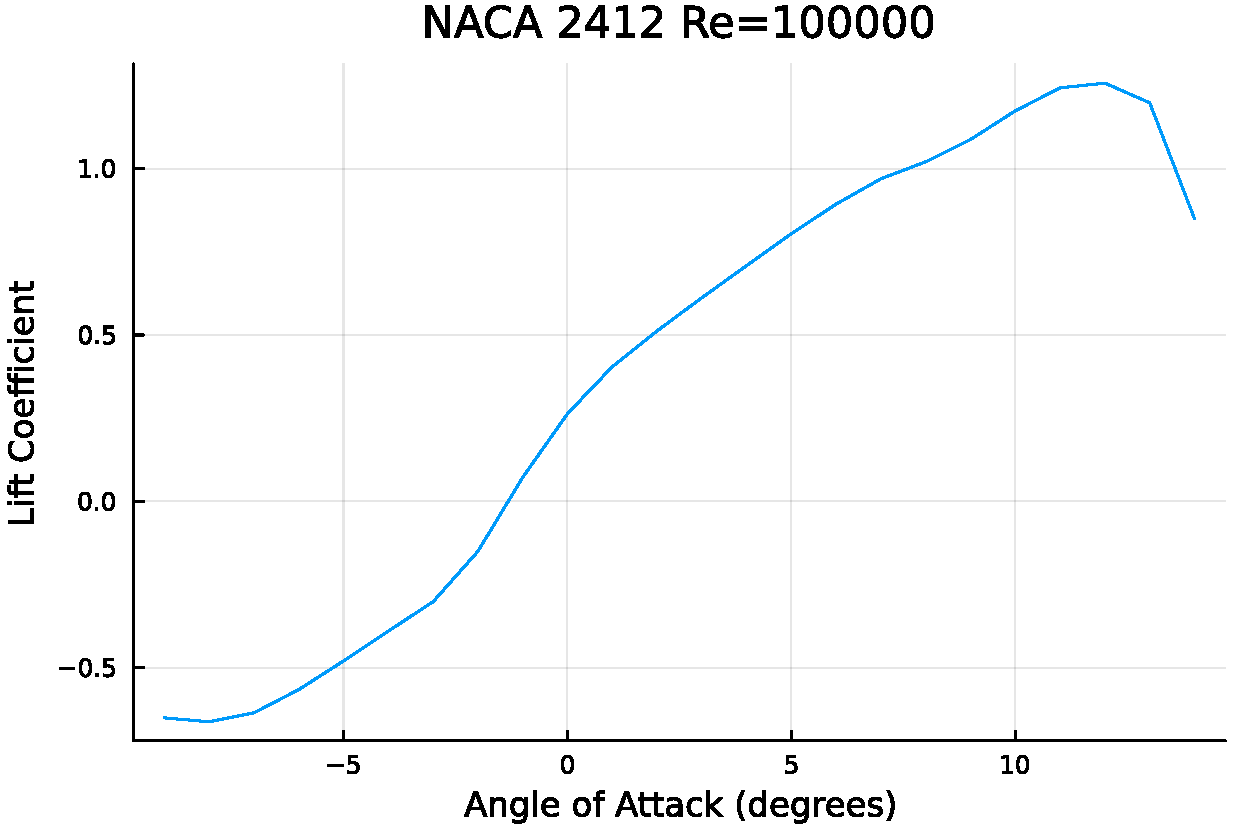
\includegraphics[width=\textwidth]{NACA 2412 Re=100000_Lift_Coefficent_Plot.pdf}
\caption{Lift of a NACA 2412 airfoil in flow with a Reynolds number of 100 thousand}
\label{fig:NACA 2412 Re=100000 Lift}
\end{minipage}
\begin{minipage}[b]{0.45\textwidth}
\centering
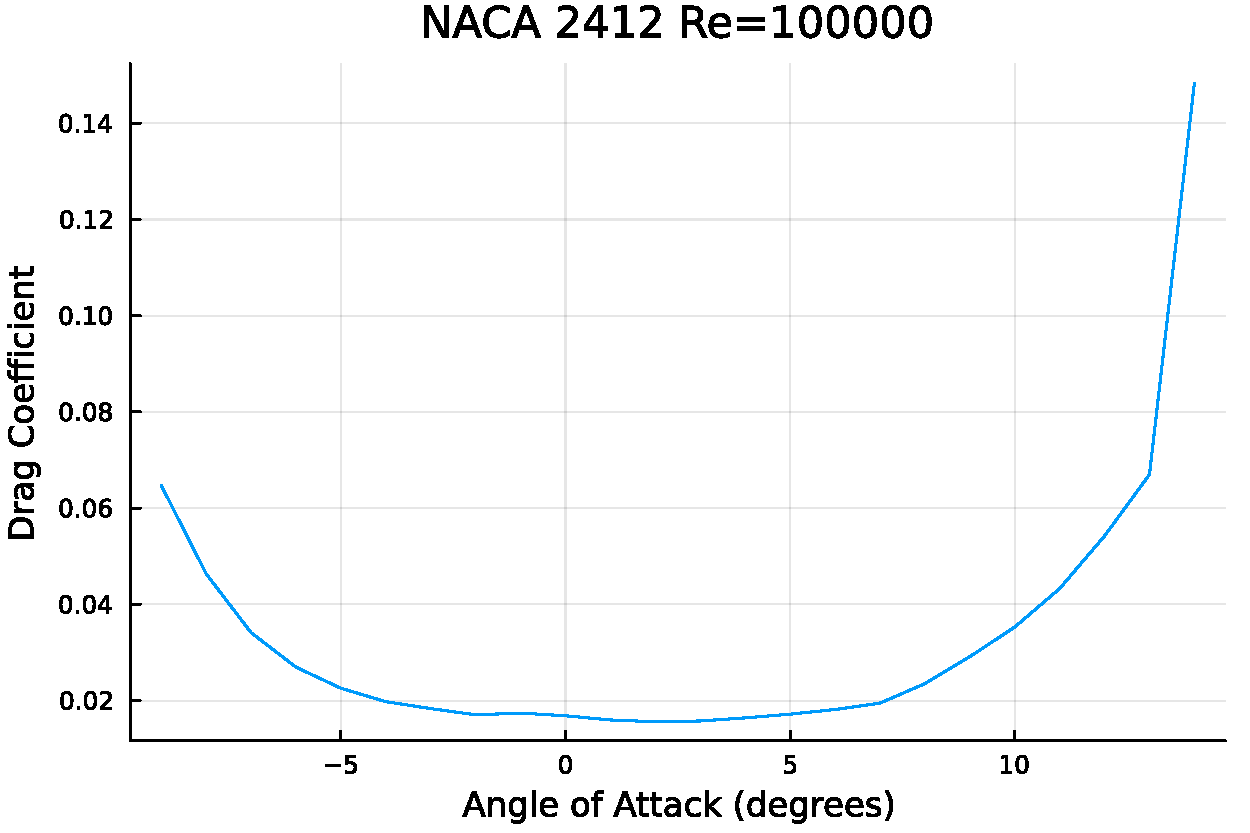
\includegraphics[width=\textwidth]{NACA 2412 Re=100000_Drag_Coefficent_Plot.pdf}
\caption{Drag of a NACA 2412 airfoil in flow with a Reynolds number of 100 thousand}
\label{fig:NACA 2412 Re=100000 Drag}
\end{minipage}
\end{figure}

\subsection{Drag Coefficient}
As shown in Figure \ref{fig:NACA 2412 Re=100000 Drag} the Drag coefficient increases with angle of attack, this change however is relatively gradual. However, once the Angle of Attack surpasses ten degrees it shoots up. This is likewise realted the stall angle of the airfoil, when the lift plummets the drag increases sharply. These forces together cause the plane to stall. To avoid insurmountable drag, the angle of attack must stay below the stall angle. Optimizing the angle of attack must consider both the total lift of the airfoil and the effect of drag and potential stalling.


\subsection{Moment Coefficient}
As shown in Figure \ref{fig:NACA 2412 Re=100000 Moment} the Moment coefficient stays relatively constant in the negative hundredths but fluctuates as lift and drag change. It increases as you move away from zero in either direction, with the minimum value near zero. Noticeably, as drag begins to sharply increase, the moment coefficient starts decreasing.

\begin{figure}[h]
    \centering
\begin{minipage}[b]{0.45\textwidth}
\centering
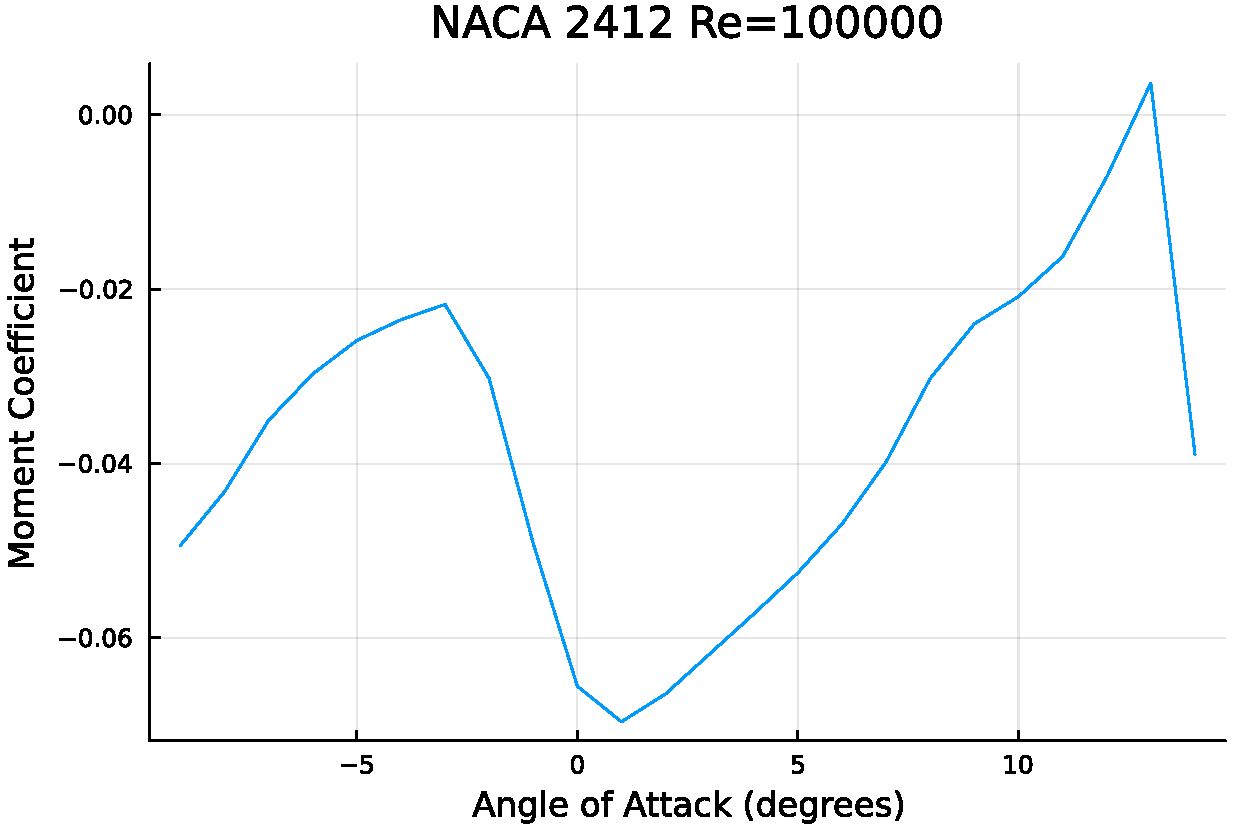
\includegraphics[width=\textwidth]{NACA 2412 Re=100000_Moment_Coefficent_Plot.pdf}
\caption{\label{fig:NACA 2412 Re=100000 Moment}Moment of a NACA 2412 Airfoil in Flow with a Reynolds Number of 100000}
\end{minipage}
\begin{minipage}[b]{0.45\textwidth}
\centering
\includegraphics[width=\textwidth]{6412:0012 Moment.jpg}
\caption{\label{fig:Xfoil Moment}Moment Coefficients found using Xfoil, third party}
\end{minipage}
\end{figure}

\section{Published Data Comparison}
Exploring how the panel method results from Xfoil compare to CFD, published Xfoil data, and experimental data for the same airfoil, we see a relatively close match. By comparing it to published data from Xfoil programs we can verify the functions are working as expected, while other comparisons help us evaluate the effectiveness of the panel method in general. In the CFD and experimental plots, there are slight differences from the Xfoil data, but the overall trends are the same.

\subsection{Xfoil Comparisons}
Looking at Xfoil data generated by others for 6412 and 0012 NACA airfoils using a Reynolds number of 1 million, we can verify if our Xfoil code is providing realistic results \cite{aerotoolbox_lift_drag_moment}. As shown by comparing Figures \ref{fig:NACA 6412 Moment} and \ref{fig:NACA 0012 Moment} with Figure \ref{fig:Xfoil Moment}, Figure \ref{fig:NACA 6412 Moment}. However, Figure \ref{fig:NACA 0012 Moment} shows good approximate values but doesn't match the data as closely. These comparisons indicate that these Xfoil functions use similar methodology to the one used by the authors of the article, yet there are potential differences in the particular NACA airfoil datasets used. This is confirmed by comparing Figure \ref{fig:NACA 0012 Moment} to a published plot from the source of the airfoil data points, showing an exact match (see Figure \ref{fig:Xfoil 0012 Moment}) \cite{naca0012h}. Comparing the drag and lift coefficients for each airfoil, we see exact matches (Comparing Figure \ref{fig:Xfoil Lift} to Figures \ref{fig:NACA 6412 Lift}, \ref{fig:NACA 0012 Lift}, \ref{fig:NACA 6412 Drag},  and \ref{fig:NACA 0012 Drag}). Confirming that this panel method code functions as expected.

\begin{figure}[h]
    \centering
\begin{minipage}[b]{0.32\textwidth}
\centering
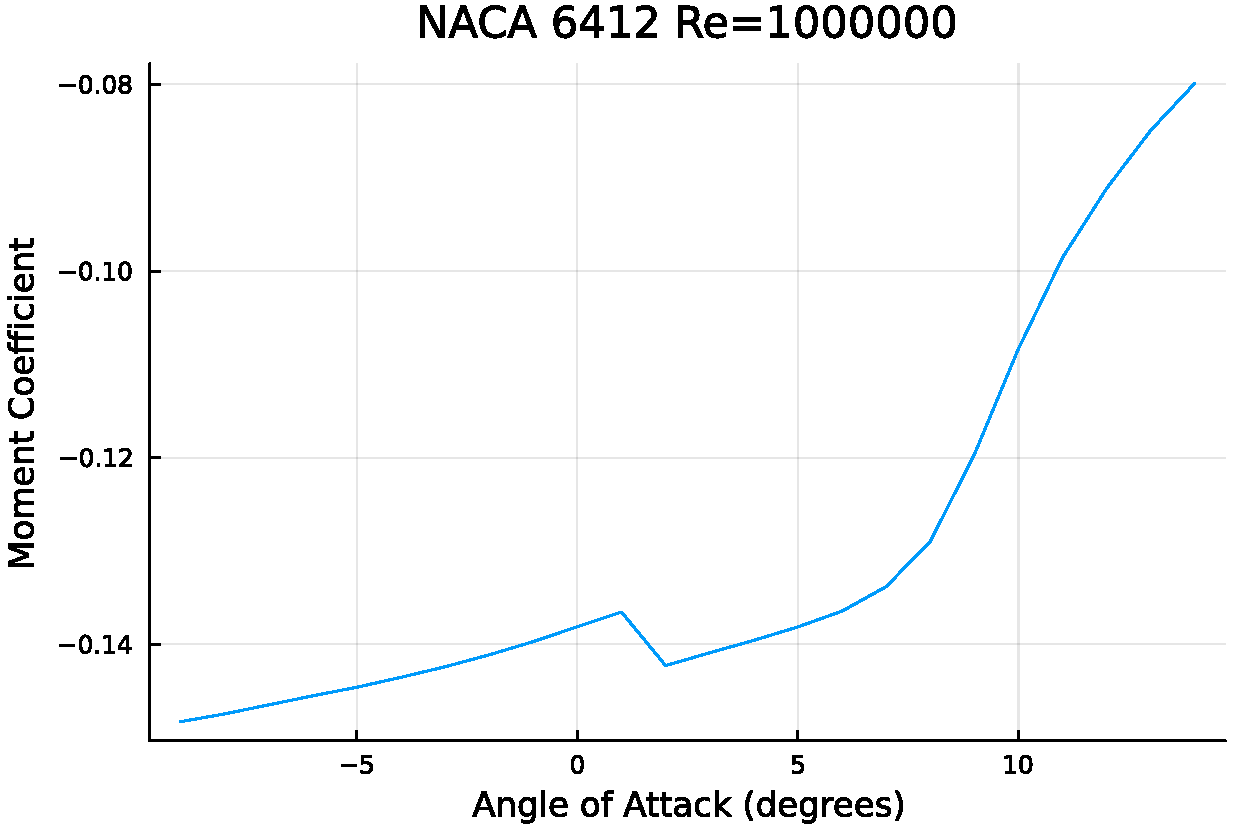
\includegraphics[width=\textwidth]{NACA 6412 Re=1000000_Moment_Coefficent_Plot.pdf}
\caption{\label{fig:NACA 6412 Moment}Moment Coefficient of a NACA 6412 Airfoil with a Reynolds number of 1 Million}
\end{minipage}
\begin{minipage}[b]{0.32\textwidth}
\centering
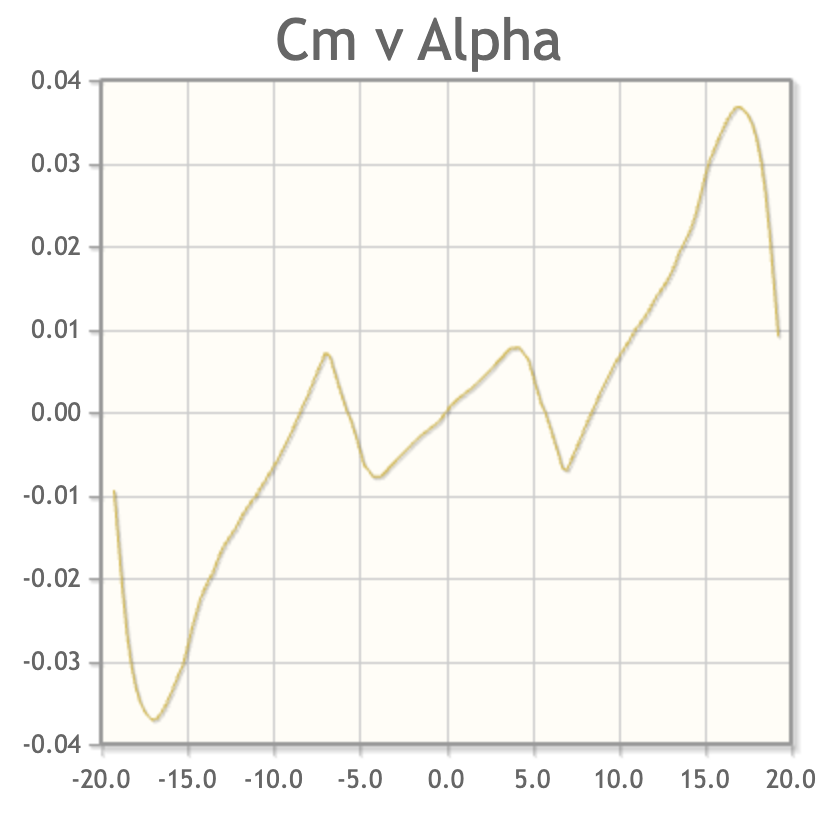
\includegraphics[width=\textwidth]{Screenshot 2024-09-11 at 7.29.20 PM.png}
\caption{\label{fig:Xfoil 0012 Moment}Moment Coefficient of a NACA 0012 Airfoil third party}
\end{minipage}
\begin{minipage}[b]{0.32\textwidth}
\centering
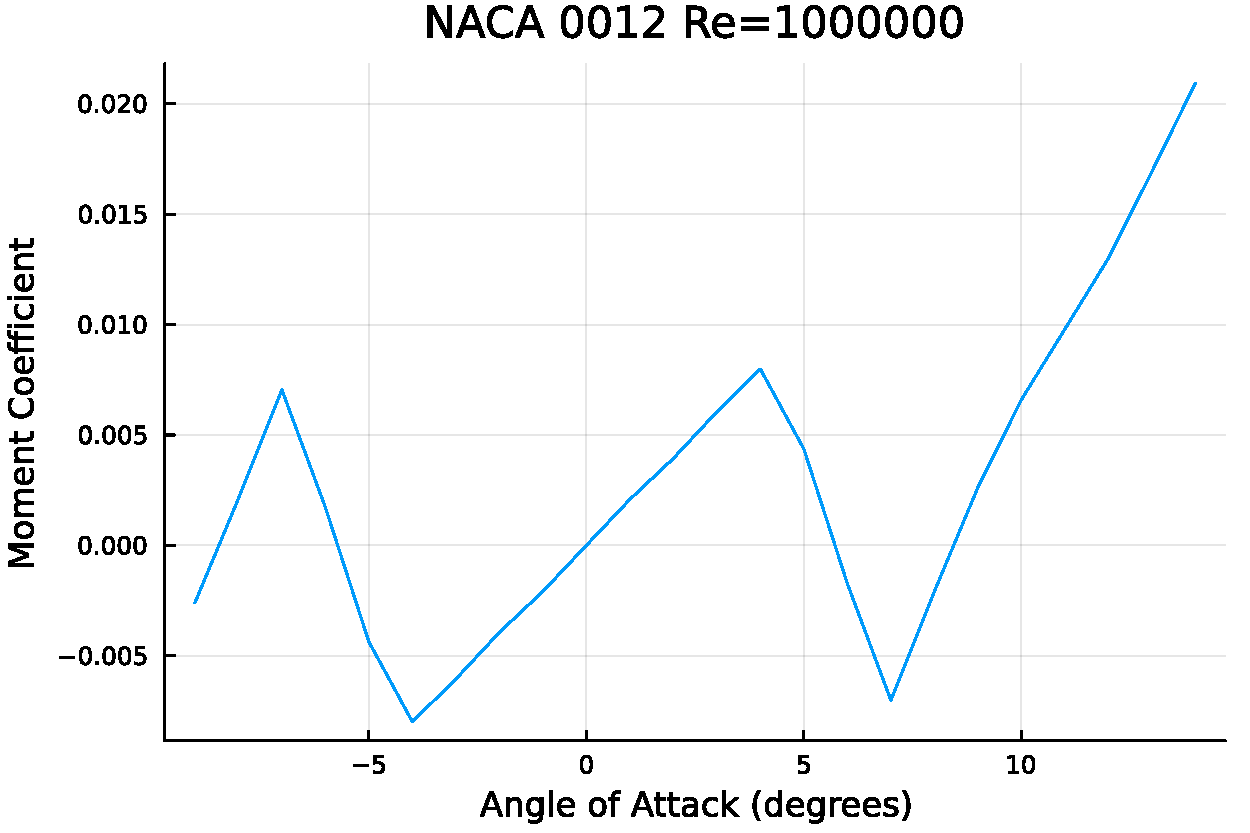
\includegraphics[width=\textwidth]{NACA 0012 Re=1000000_Moment_Coefficent_Plot.pdf}
\caption{\label{fig:NACA 0012 Moment}Moment Coefficient of a NACA 0012 Airfoil with a Reynolds number of 1 Million}
\end{minipage}
\end{figure}

\begin{figure}[h]
    \centering
\begin{minipage}[b]{0.66\textwidth}
\centering
\includegraphics[width=\textwidth]{6412:0012 Lift.jpg}
\caption{\label{fig:Xfoil Lift}Lift Coefficients found using Xfoil, third party}
\end{minipage}
\begin{minipage}[b]{0.32\textwidth}
\centering
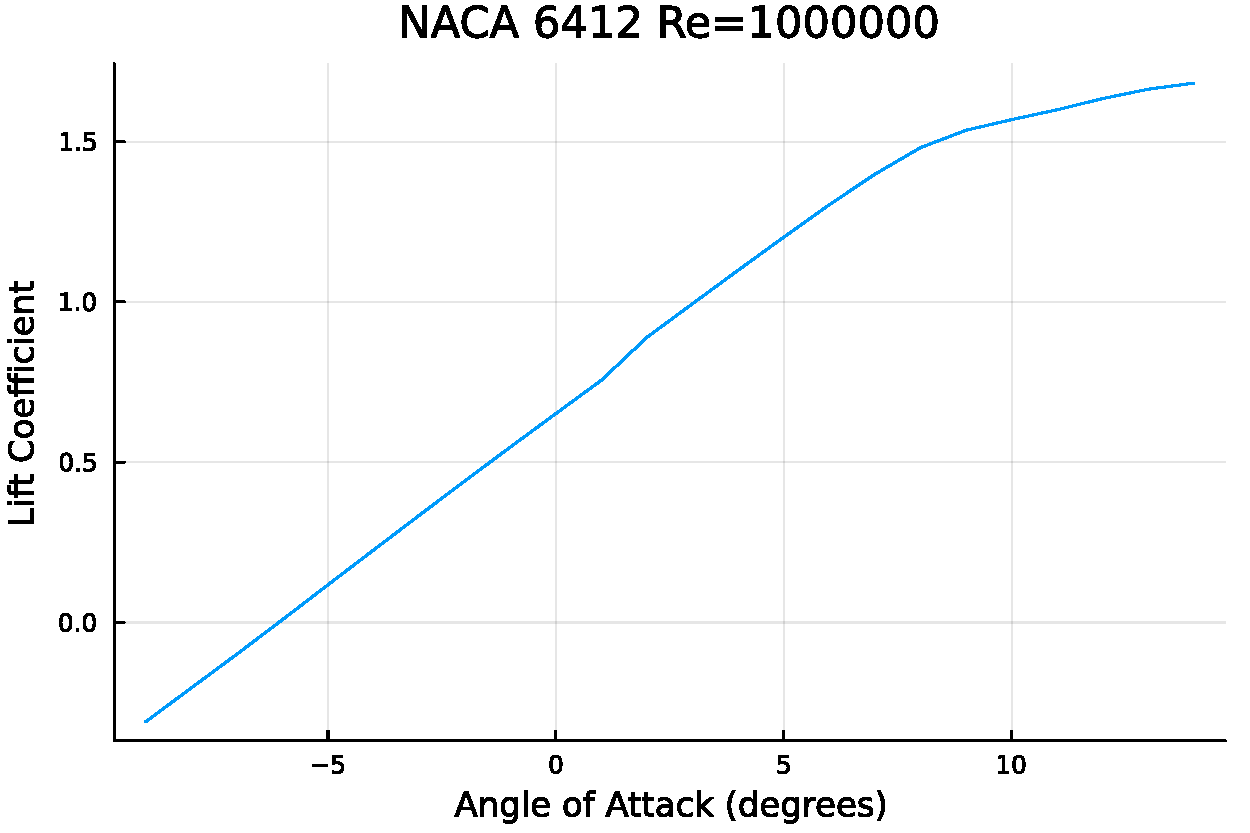
\includegraphics[width=\textwidth]{NACA 6412 Re=1000000_Lift_Coefficent_Plot.pdf}
\caption{\label{fig:NACA 6412 Lift}Lift Coefficient of a NACA 6412 Airfoil with a Reynolds number of 1 Million}
\end{minipage}
\end{figure}

\begin{figure}[h]
    \centering
\begin{minipage}[b]{0.32\textwidth}
\centering
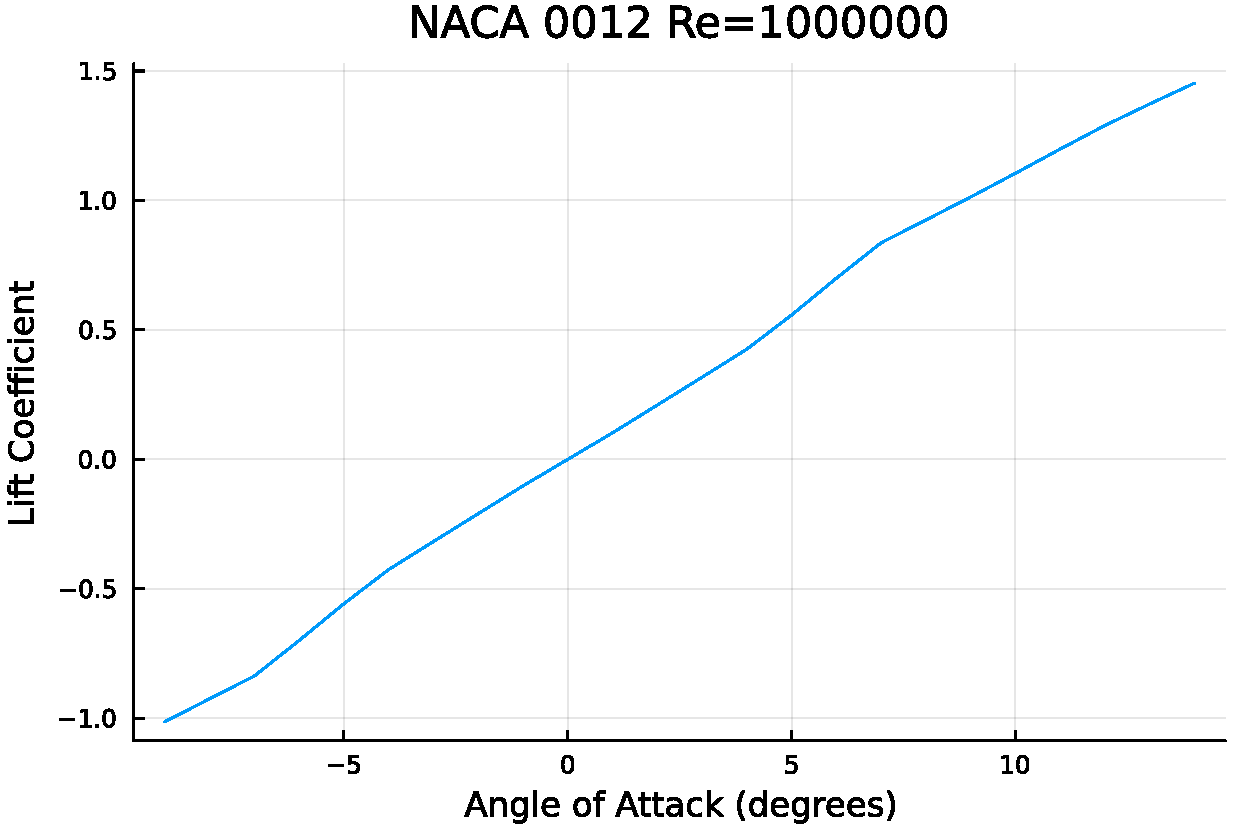
\includegraphics[width=\textwidth]{NACA 0012 Re=1000000_Lift_Coefficent_Plot.pdf}
\caption{\label{fig:NACA 0012 Lift}Lift Coefficient of a NACA 0012 Airfoil with a Reynolds number of 1 Million}
\end{minipage}
\begin{minipage}[b]{0.32\textwidth}
\centering
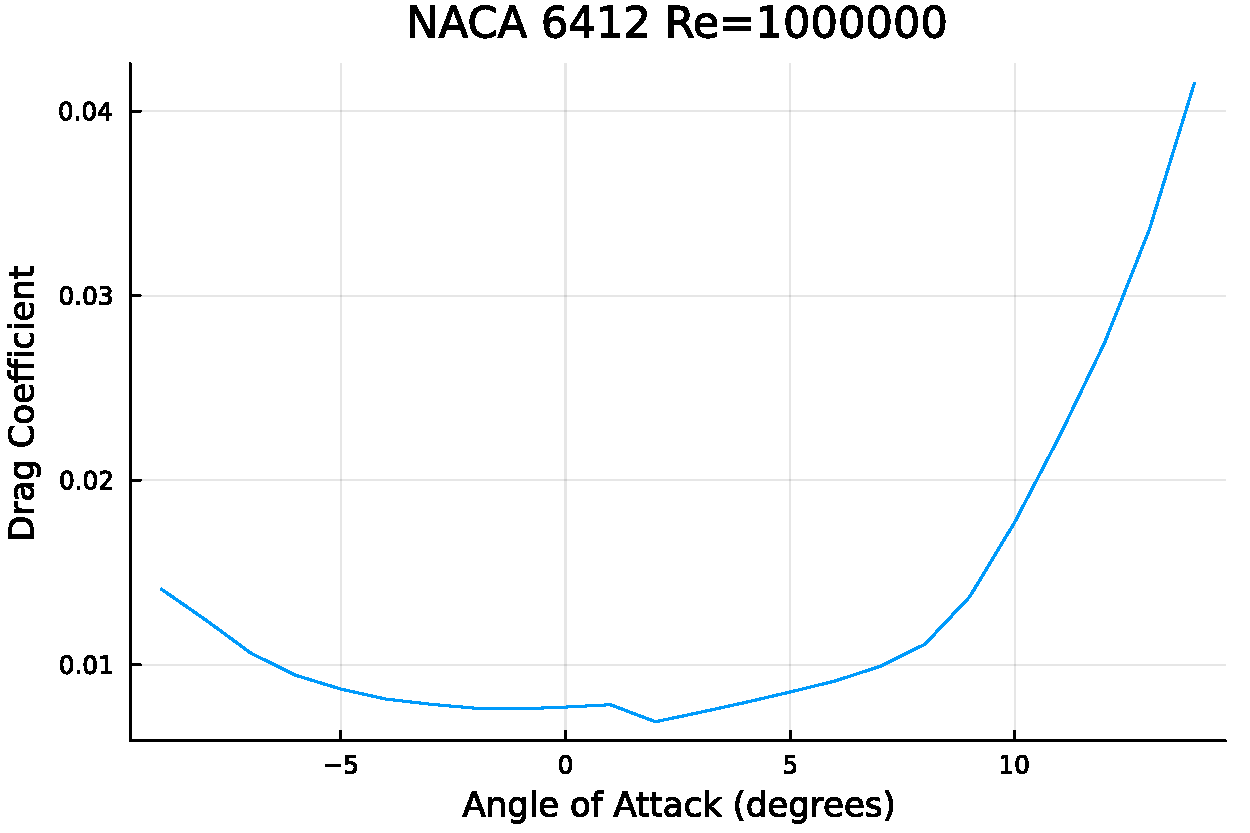
\includegraphics[width=\textwidth]{NACA 6412 Re=1000000_Drag_Coefficent_Plot.pdf}
\caption{\label{fig:NACA 6412 Drag}Drag Coefficient of a NACA 6412 Airfoil with a Reynolds number of 1 Million}
\end{minipage}
\begin{minipage}[b]{0.32\textwidth}
\centering
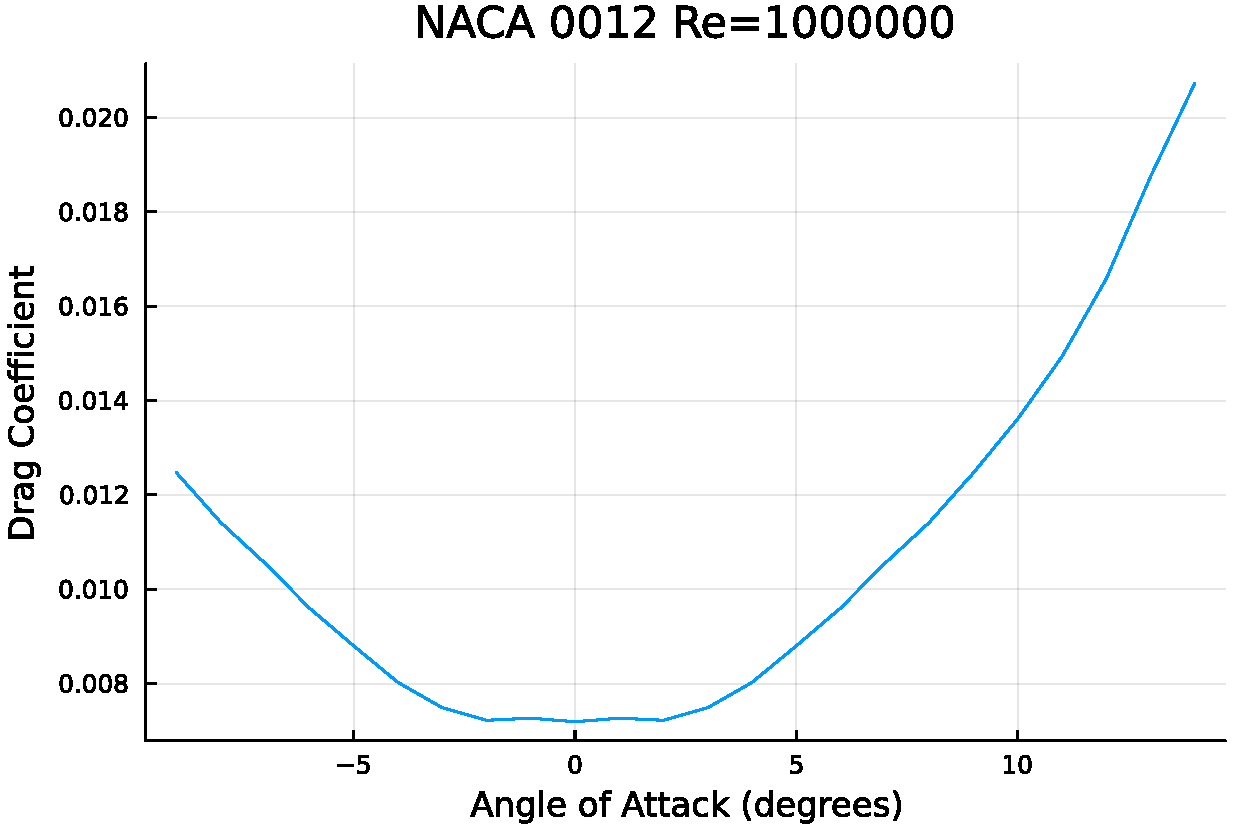
\includegraphics[width=\textwidth]{NACA 0012 Re=1000000_Drag_Coefficent_Plot.pdf}
\caption{\label{fig:NACA 0012 Drag}Drag Coefficient of a NACA 0012 Airfoil with a Reynolds number of 1 Million}
\end{minipage}
\end{figure}

\subsection{CFD Comparisons}
Looking at an article published that used CFD on a NACA 2412, we see an additional match \cite{KULSHRESHTHA20201638}. Comparing Figure \ref{fig:NACA 2412 Re=100000 Drag} to Figure \ref{fig:CFD NACA 2412 Drag} you can see the similar trend of sharp uptakes in drag as the stall angle is approached and passed. Similarly, there is a similar linear portion up to a stall angle in Figure \ref{fig:NACA 2412 Re=100000 Lift} and Figure \ref{fig:CFD NACA 2412 Lift}. However the exact values in these differ slightly, likely mostly due to a difference in Reynolds number since the one used in the CFD calculations wasn't readily available.

\begin{figure}[h]
    \centering
\begin{minipage}[b]{0.45\textwidth}
\centering
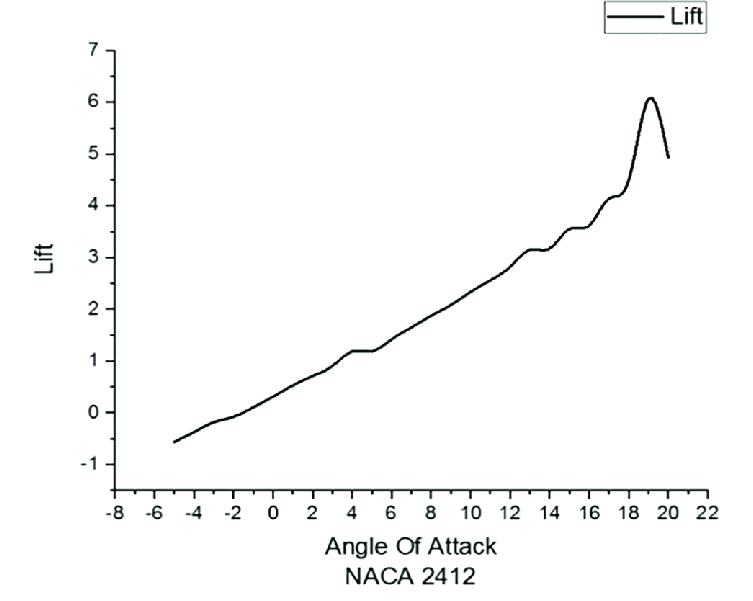
\includegraphics[width=\textwidth]{CFD 2412 Lift.png}
\caption{\label{fig:CFD NACA 2412 Lift}Lift Coefficient of a NACA 2412 Airfoil Calculated with Computational Fluid Dynamics}
\end{minipage}
\begin{minipage}[b]{0.45\textwidth}
\centering
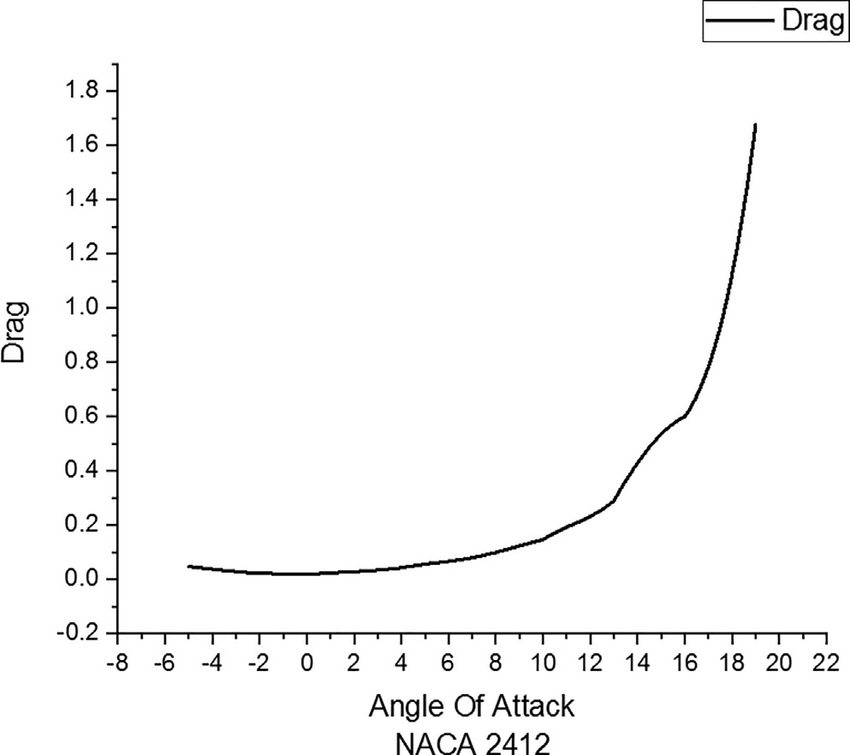
\includegraphics[width=\textwidth]{CFD 2412 Drag.png}
\caption{\label{fig:CFD NACA 2412 Drag}Drag Coefficient of a NACA 2412 Airfoil Calculated with Computational Fluid Dynamics}
\end{minipage}
\end{figure}

\subsection{Experimental Data Comparisons}

To compare with experimental data, I used a study conducted by NASA \cite{anderson1994simplified} in the 90's testing airfoils in a wind tunnel to verify the Xfoil data. Comparing Figures \ref{fig:NACA 2412 Lift} and \ref{fig:NACA 2412 Drag} to Figures \ref{fig:Exp 2412 Lift} and \ref{fig:CFD NACA 2412 Drag} we see extremely similar patterns and stall angles. The values of the coefficients for those angle of attacks are also close, showing a good match between the experimental data and the Xfoil-generated plots.

\begin{figure}[h]
    \centering
\begin{minipage}[b]{0.3\textwidth}
\centering
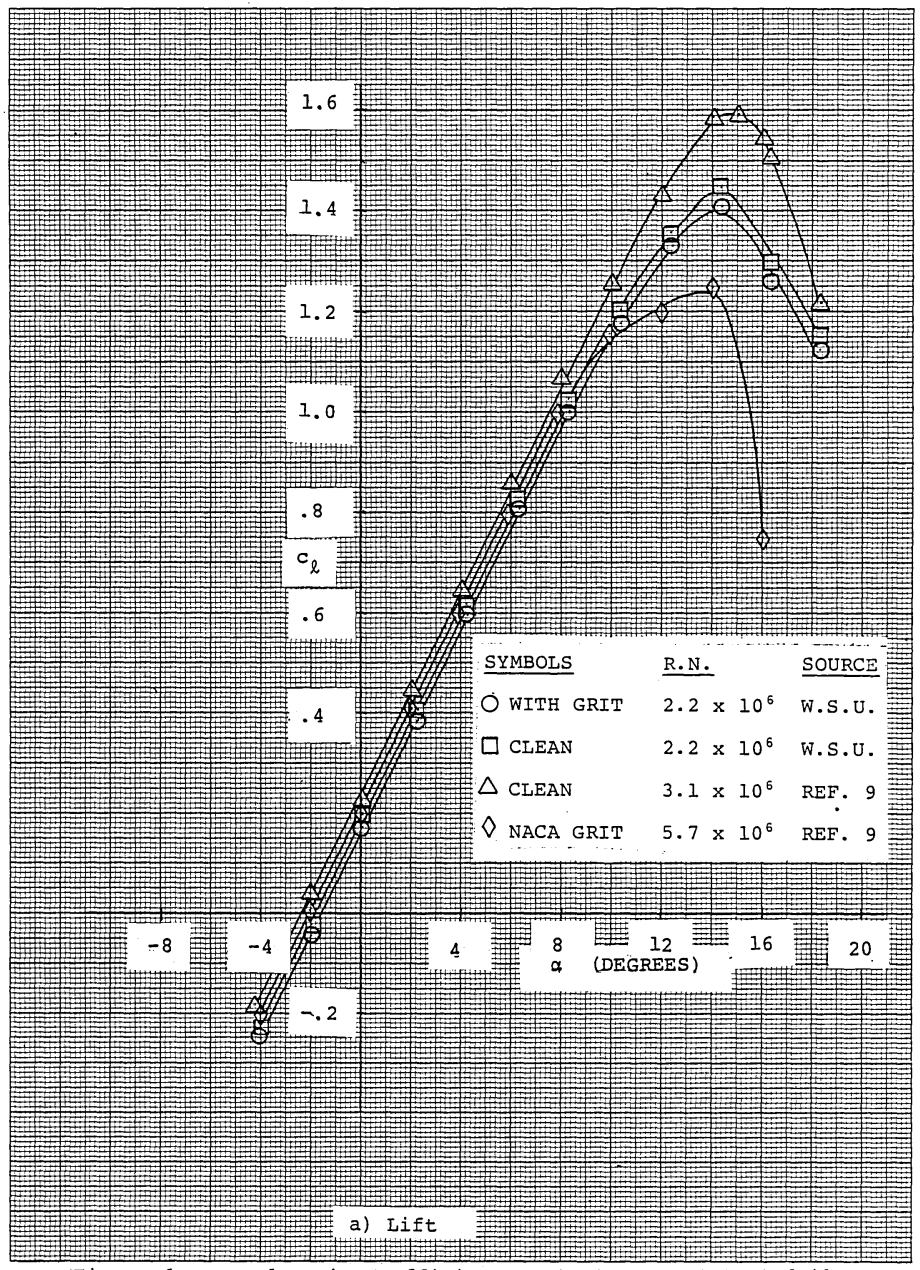
\includegraphics[width=\textwidth]{Screenshot 2024-09-10 at 10.59.39 PM.png}
\caption{\label{fig:Exp 2412 Lift}Lift Coefficient of a NACA 2412 Airfoil Determined Experimentally}
\end{minipage}
\begin{minipage}[b]{0.69\textwidth}
\centering
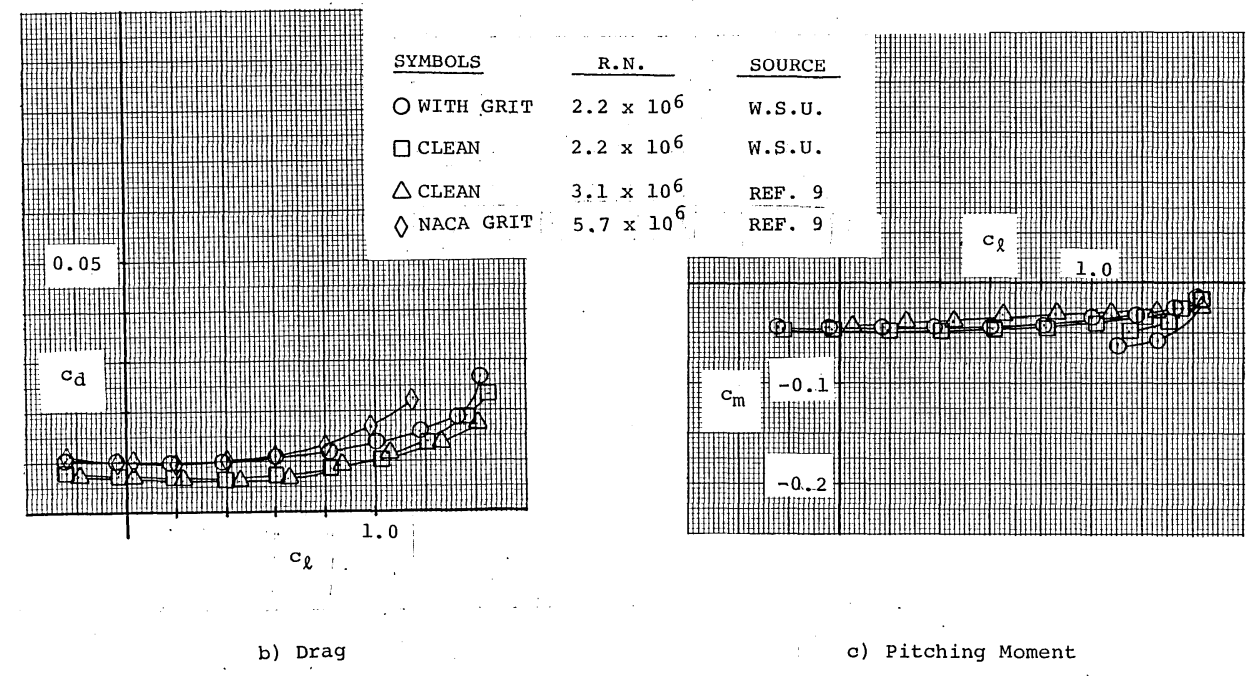
\includegraphics[width=\textwidth]{Screenshot 2024-09-10 at 10.59.51 PM.png}
\caption{\label{fig:Exp 2412 Drag}Drag Coefficient of a NACA 2412 Airfoil Determined Experimentally}
\end{minipage}
\end{figure}

\begin{figure}[h]
    \centering
\begin{minipage}[b]{0.45\textwidth}
\centering
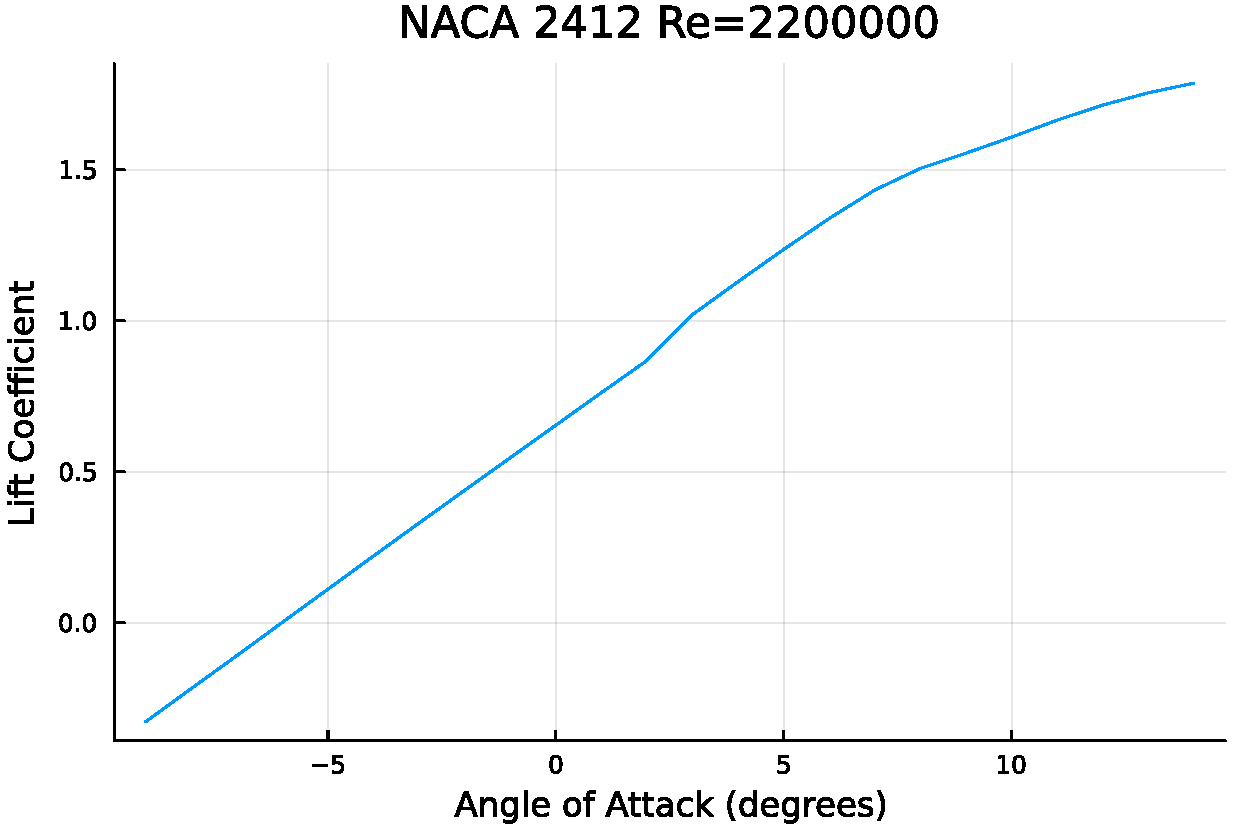
\includegraphics[width=\textwidth]{NACA 2412 Re=2200000_Lift_Coefficent_Plot.pdf}
\caption{\label{fig:NACA 2412 Lift}Lift Coefficient of a NACA 2412 Airfoil with a Reynolds Number of 2.2 Million}
\end{minipage}
\begin{minipage}[b]{0.45\textwidth}
\centering
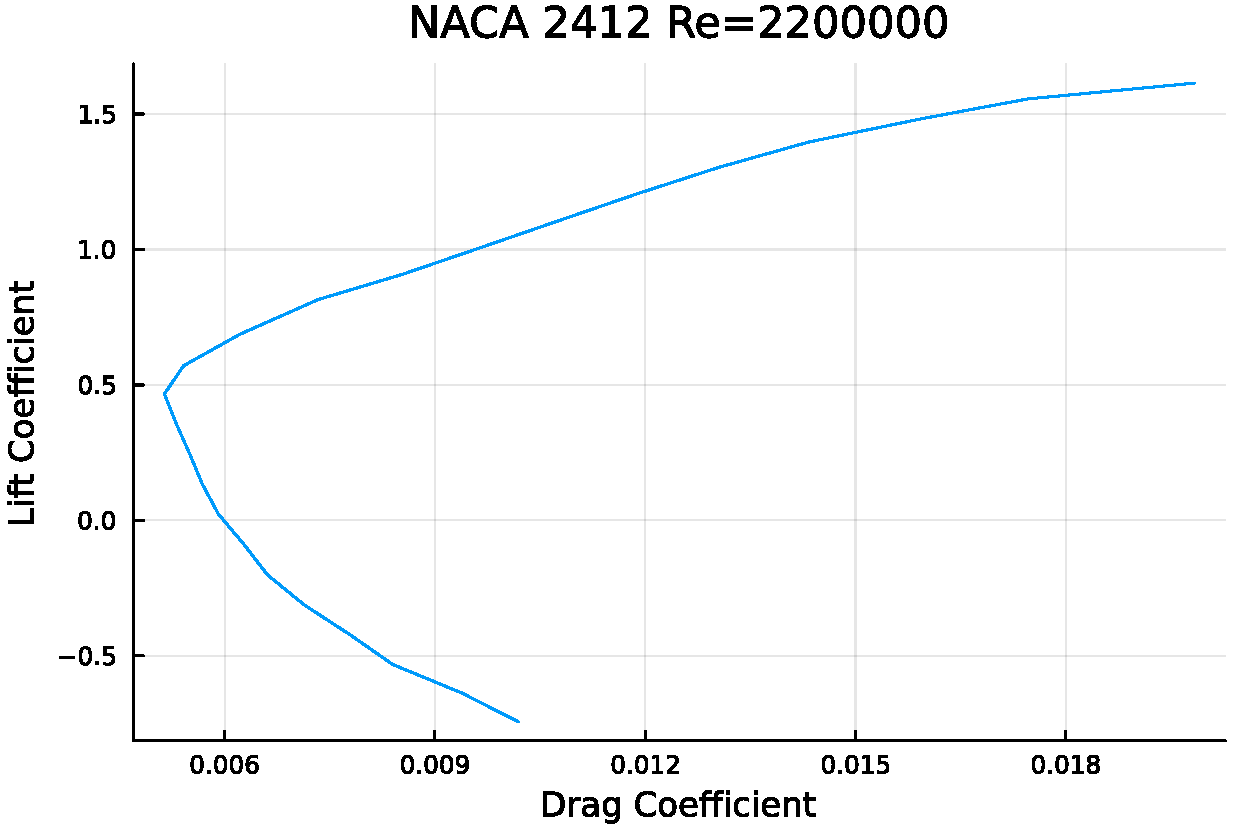
\includegraphics[width=\textwidth]{NACA 2412 Re=2200000_Drag_vs_Lift_Coefficent_Plot.pdf}
\caption{\label{fig:NACA 2412 Drag}Drag vs Lift Coefficients of a NACA 2412 Airfoil with a Reynolds Number of 2.2 Million}
\end{minipage}
\end{figure}

\begin{figure}[h]
    \centering
\begin{minipage}[b]{0.32\textwidth}
\centering
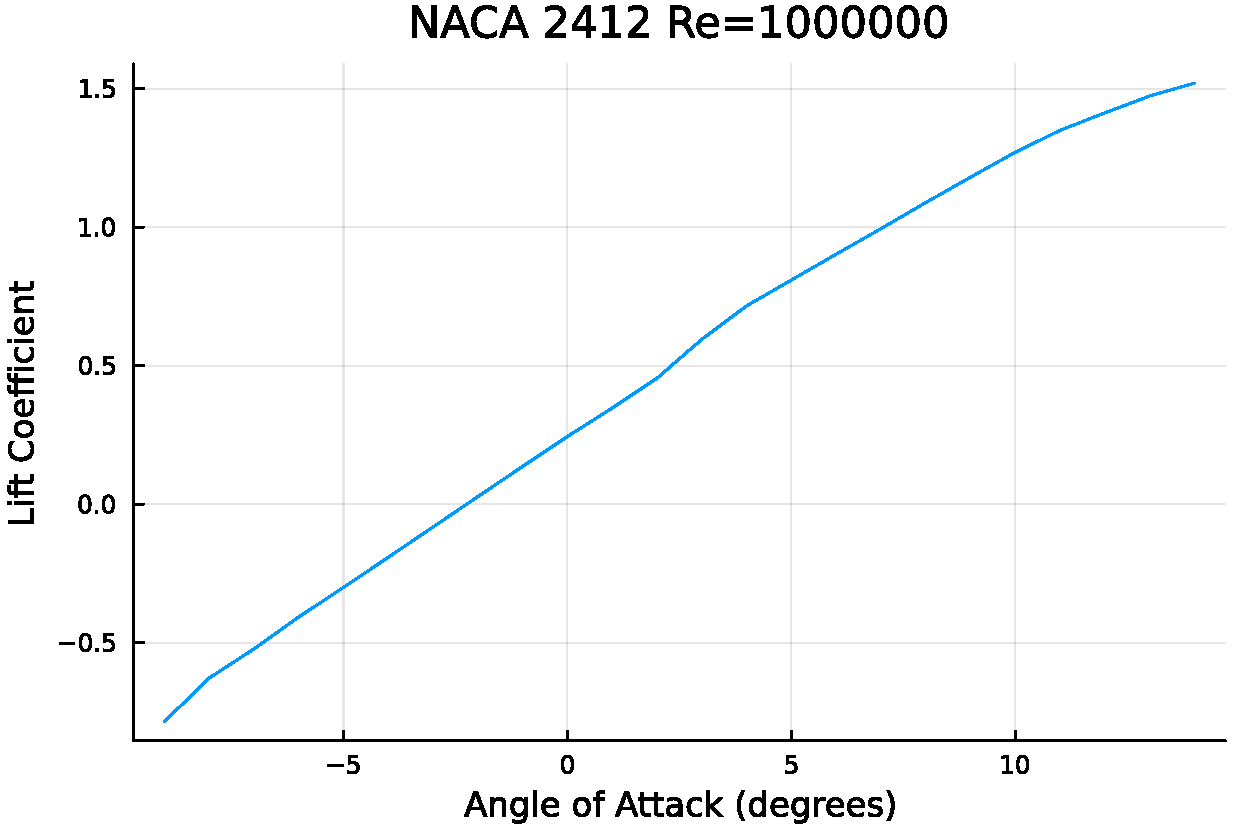
\includegraphics[width=\textwidth]{NACA 2412 Re=1000000_Lift_Coefficent_Plot.pdf}
\caption{Lift of a NACA 2412 Airfoil in Flow with a Reynolds Number of 1 Million}
\label{fig:NACA 2412 Re=1000000 Lift}
\end{minipage}
\begin{minipage}[b]{0.32\textwidth}
\centering
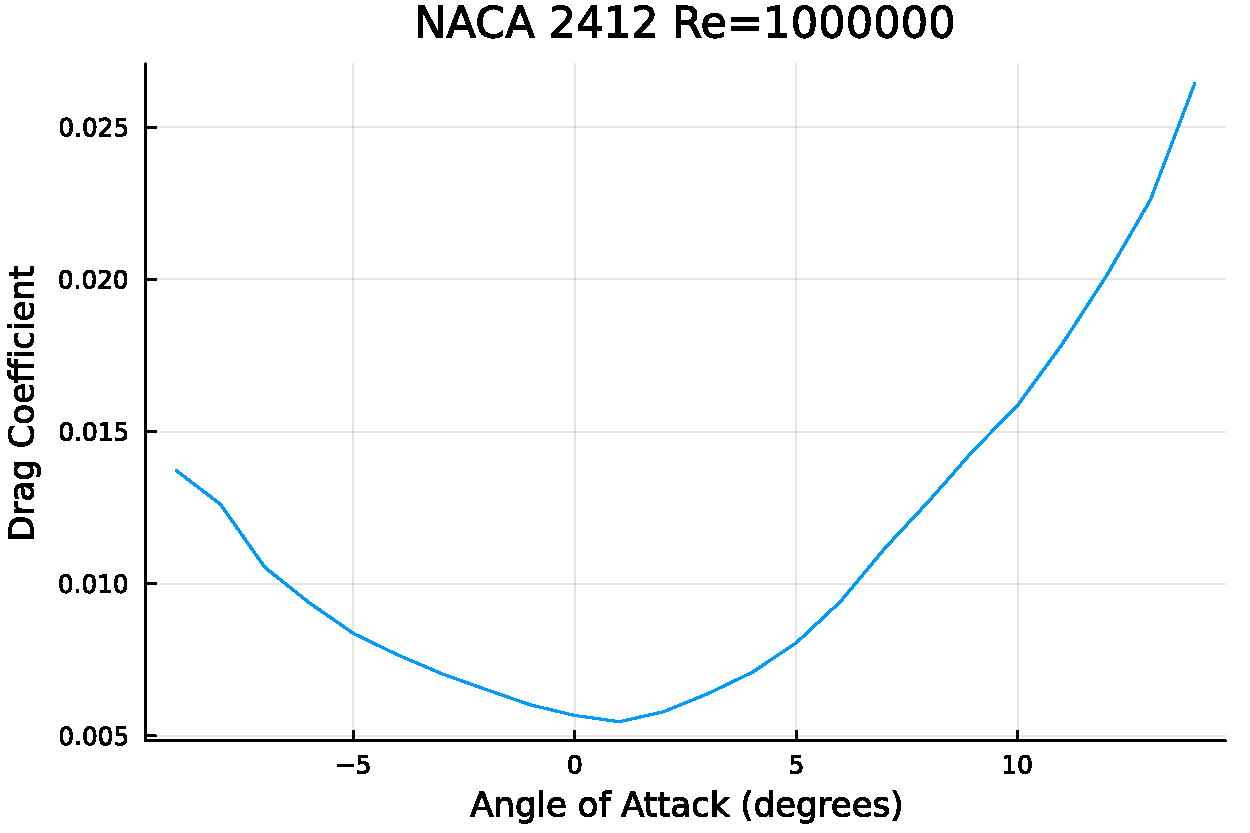
\includegraphics[width=\textwidth]{NACA 2412 Re=1000000_Drag_Coefficent_Plot.pdf}
\caption{Drag of a NACA 2412 Airfoil in Flow with a Reynolds Number of 1 Million}
\label{fig:NACA 2412 Re=1000000 Drag}
\end{minipage}
\begin{minipage}[b]{0.32\textwidth}
\centering
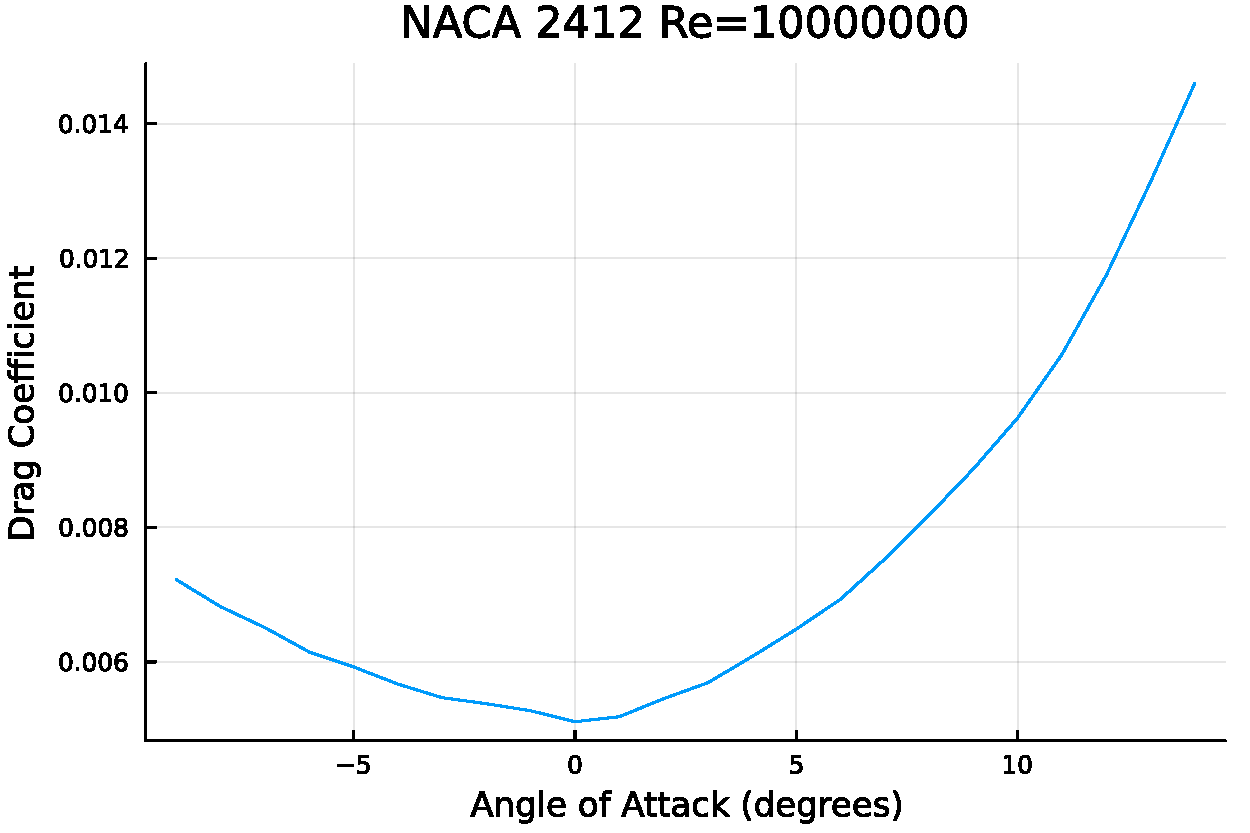
\includegraphics[width=\textwidth]{NACA 2412 Re=10000000_Drag_Coefficent_Plot.pdf}
\caption{\label{fig:NACA 2412 Drag Re=10000000}Drag Coefficient of a NACA 2412 Airfoil with a Reynolds Number of 10 Million}
\end{minipage}
\end{figure}

\subsection{Comparison Conclusion}
The Xfoil method aligns well with real data, CFD simulations, and other Xfoil programs. Overall, the panel method is accurate in estimating the lift, drag, and moment coefficients of a NACA airfoil for a given angle of attack and Reynolds number.

\section{Reynolds Number Effect}

The Reynolds number is a dimensionless value that represents the ratio of inertial to viscous forces. It characterizes the behavior of a fluid as it flows over a plate and determines if the flow is turbulent or laminar, affecting the lift, drag, and moment of the plane.

\subsection{Lift Coefficient}

As the Reynolds number increases the flow becomes more turbulent. Turbulent flow can follow sharper curves for longer, allowing the airfoil to handle more extreme angles of attack before stalling, as seen by comparing Figures \ref{fig:NACA 2412 Re=1000000 Lift} and \ref{fig:NACA 2412 Lift}.

\subsection{Drag Coefficient}

At low angles of attack, the drag coefficient is similar, but it increases much quicker with higher Reynolds numbers due to more eddies and vortices. This increases boundary layer thickness which increases skin friction drag, and causes larger pressure differences increasing the pressure drag. This effect on the drag coefficient can be seen by comparing Figures \ref{fig:NACA 2412 Re=1000000 Drag} and \ref{fig:NACA 2412 Drag Re=10000000}.

\subsection{Moment Coefficient}

As observed in Figures \ref{fig:NACA 2412 Moment Re=1000000} and \ref{fig:NACA 2412 Moment Re=10000000} in Appendix \ref{sec:zero_appendix}, the moment coefficient becomes more level and less responsive to changes in the angle of attack. This could be due to increased mixing, delayed separation of more turbulent flow, or perhaps the increased turbulence causes a more even pressure distribution.

\section{Effect of Airfoil Shape}
The shape of the airfoil significantly affects fluid flow impacting the lift, drag, and moment coefficients.
\subsection{Camber}
Camber, the curve or asymmetry of the wing, is one way to manipulate airfoil shape. It is the maximum distance between the chord line and a line equidistant between the upper and lower surfaces. For a symmetrical airfoil the camber is 0. 
\subsubsection{Lift to Drag Ratio}

Increased camber results in a positive shift in the lift to drag ratio, with greater periods of low drag and more rapid increases to higher drag coefficients. This can be seen by comparing Figures \ref{fig:NACA 0012 Lift Drag}, \ref{fig:NACA 2412 Lift Drag} and \ref{fig:NACA 6412 Lift Drag} in Appendix \ref{sec:first_appendix}.

\subsubsection{Lift Curve Slop}

The slope of the lift coefficient versus the angle of attack increases with increased camber, as shown by comparing Figures \ref{fig:NACA 2412 Re=1000000 Lift}, \ref{fig:NACA 6412 Lift} and \ref{fig:NACA 0012 Lift}.


\subsection{Thickness}
Thickness, the maximum distance between the upper and lower surfaces of the airfoil perpendicular to the chord line, is another way we can manipulate the shape of the airfoil.

\subsubsection{Lift to Drag Ratio}
For thinner airfoils the lift coefficient plateaus or maxes out sooner when compared to the drag. This can be seen by comparing Figures \ref{fig:NACA 2408 Drag Lift}, \ref{fig:NACA 2410 Drag Lift}, \ref{fig:NACA 2412 Lift Drag} and \ref{fig:NACA 2414 Drag Lift} in Appendix \ref{sec:second_appendix}.

\subsubsection{Lift Curve Slope}
Thickness has little effect on the slope of the lift curve. However, it does seem to postpone the stall angle, shown by comparing Figures \ref{fig:NACA 2408 Lift}, \ref{fig:NACA 2410 Lift}, \ref{fig:NACA 2412 Re=1000000 Lift} and \ref{fig:NACA 2414 Lift} in Appendix \ref{sec:third_appendix}.

\bibliographystyle{alpha}
\bibliography{sample}

\clearpage
\appendix

\section{Camber Lift to Drag Ratio Plots}
\label{sec:zero_appendix}

\begin{figure}[h]
    \centering
\begin{minipage}[b]{0.45\textwidth}
\centering
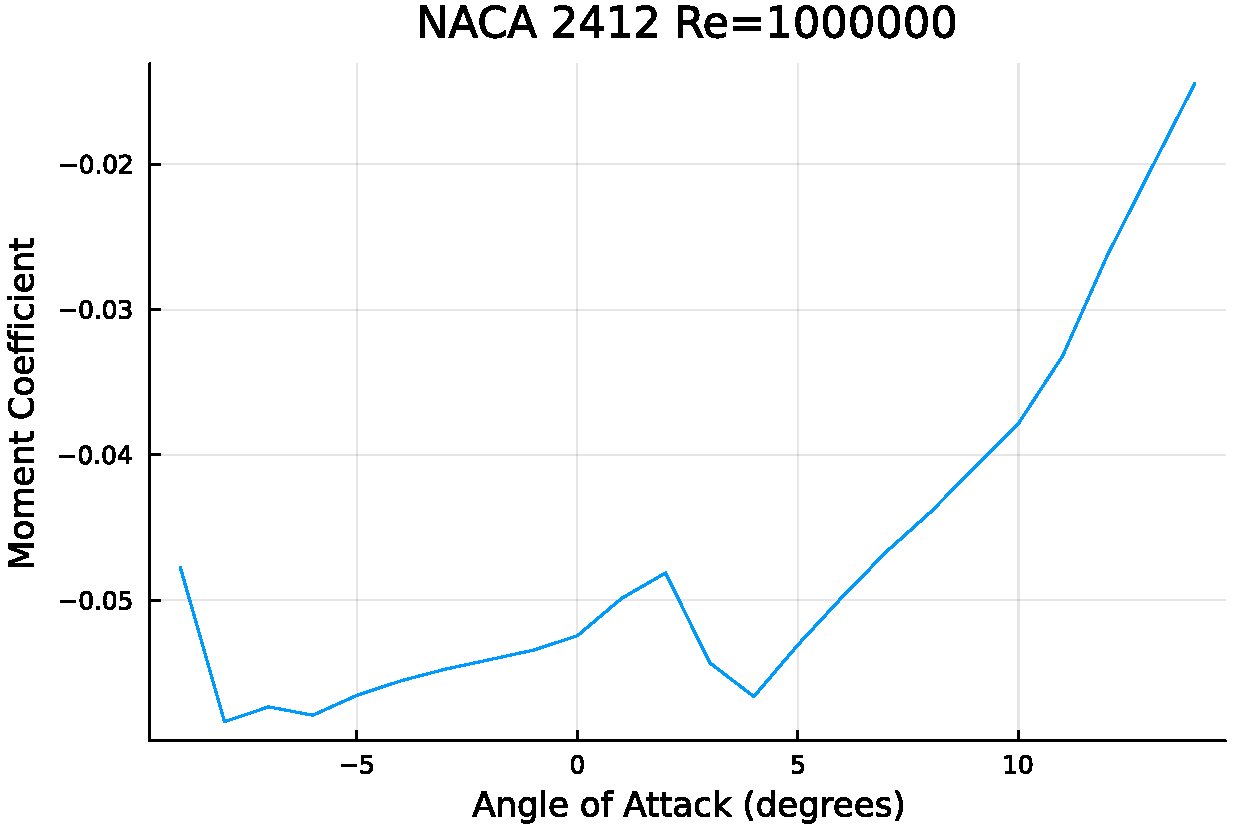
\includegraphics[width=\textwidth]{NACA 2412 Re=1000000_Moment_Coefficent_Plot.pdf}
\caption{\label{fig:NACA 2412 Moment Re=1000000}Moment Coefficient of a NACA 2412 Airfoil with a Reynolds Number of 1 Million}
\end{minipage}
\begin{minipage}[b]{0.45\textwidth}
\centering
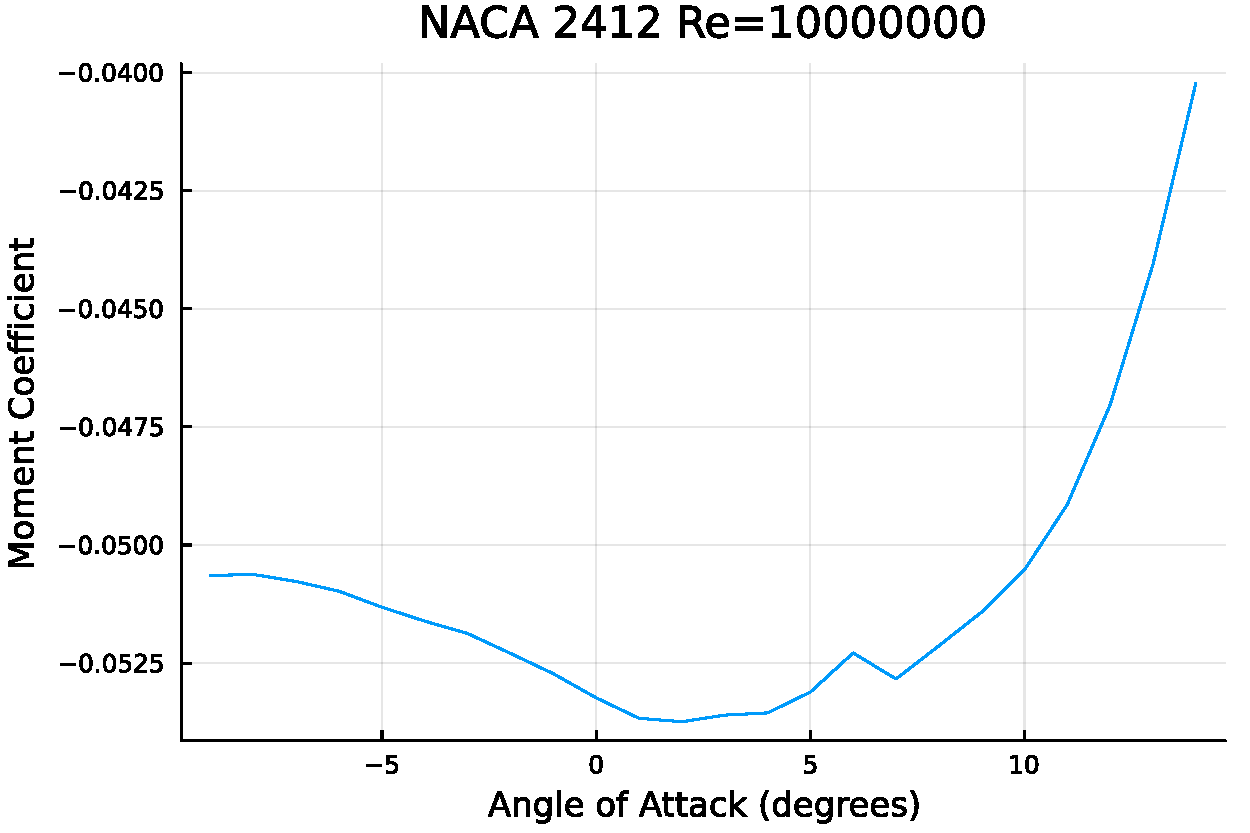
\includegraphics[width=\textwidth]{NACA 2412 Re=10000000_Moment_Coefficent_Plot.pdf}
\caption{\label{fig:NACA 2412 Moment Re=10000000}Moment Coefficient of a NACA 2412 Airfoil with a Reynolds Number of 10 Million}
\end{minipage}
\end{figure}

\section{Camber Lift to Drag Ratio Plots}
\label{sec:first_appendix}

\begin{figure}[h]
    \centering
\begin{minipage}[b]{0.32\textwidth}
\centering
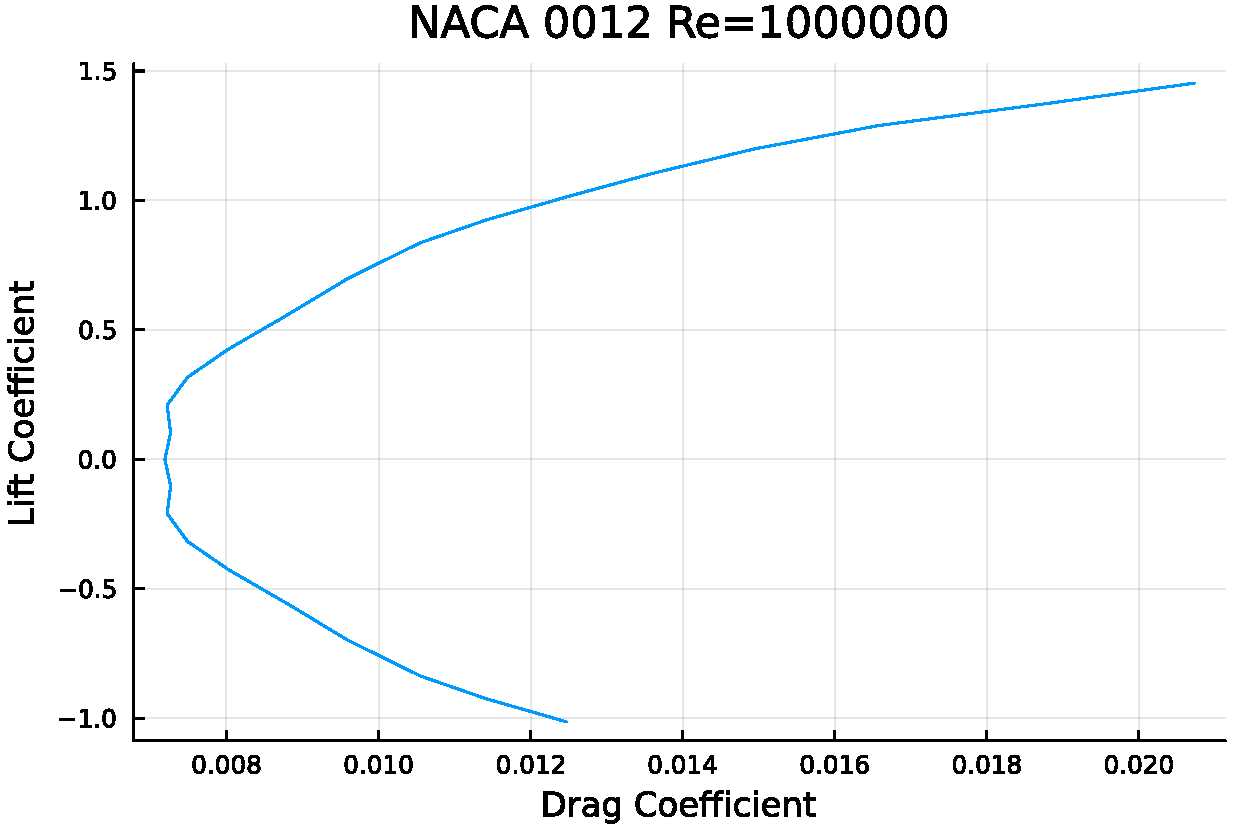
\includegraphics[width=\textwidth]{NACA 0012 Re=1000000_Drag_vs_Lift_Coefficent_Plot.pdf}
\caption{\label{fig:NACA 0012 Lift Drag}Drag vs Lift Profile NACA 0012}
\end{minipage}
\begin{minipage}[b]{0.32\textwidth}
\centering
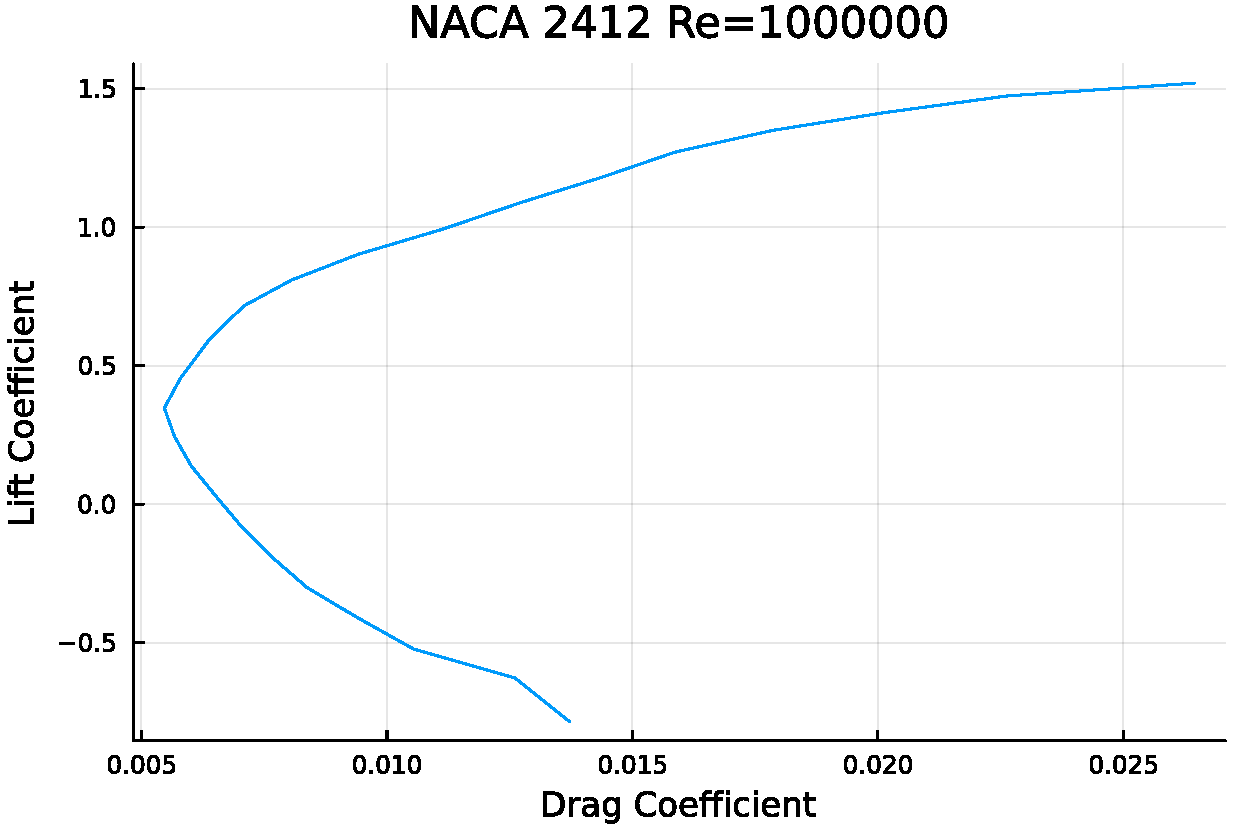
\includegraphics[width=\textwidth]{NACA 2412 Re=1000000_Drag_vs_Lift_Coefficent_Plot.pdf}
\caption{\label{fig:NACA 2412 Lift Drag}Drag vs Lift Profile NACA 2412 with a Reynolds number of 1 Million}
\end{minipage}
\begin{minipage}[b]{0.32\textwidth}
\centering
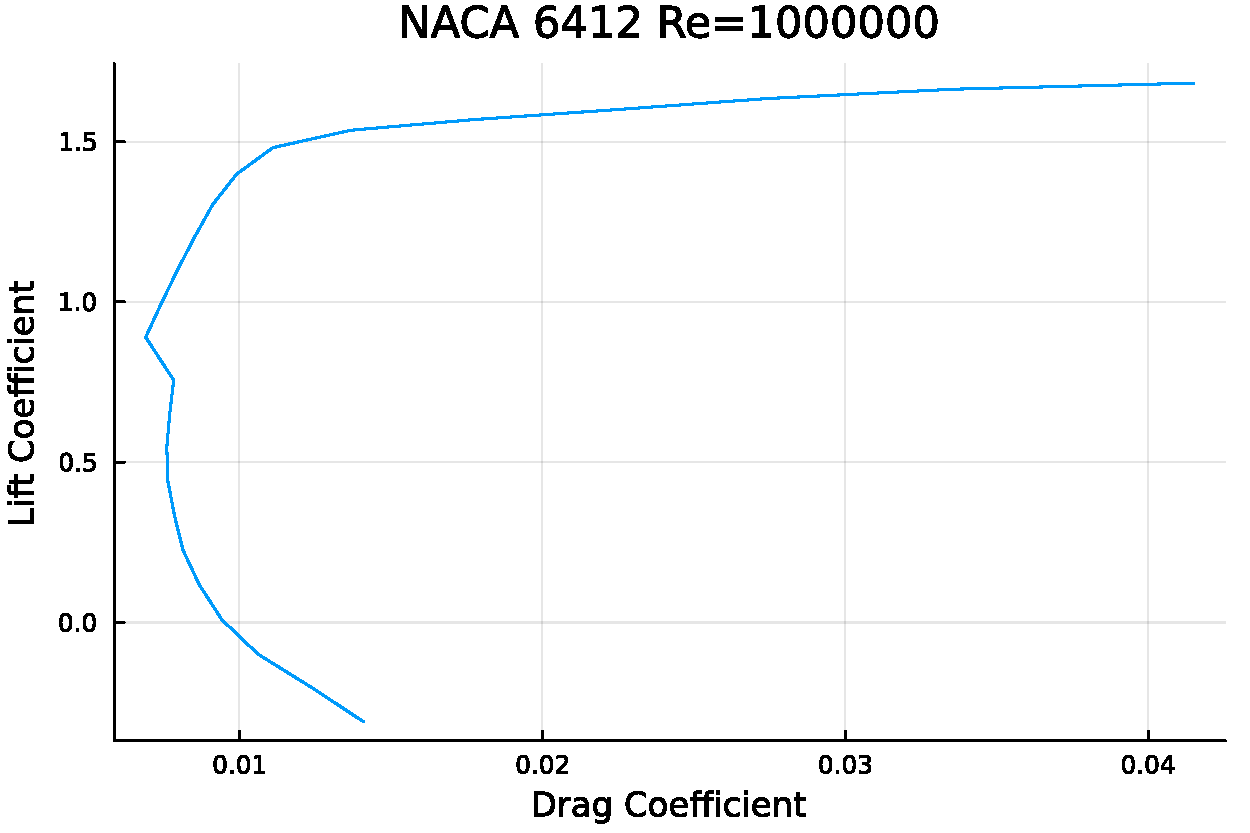
\includegraphics[width=\textwidth]{NACA 6412 Re=1000000_Drag_vs_Lift_Coefficent_Plot.pdf}
\caption{\label{fig:NACA 6412 Lift Drag}Drag vs Lift Profile NACA 6412}
\end{minipage}
\end{figure}

\section{Thickness Lift to Drag Ratio Plots}
\label{sec:second_appendix}

\begin{figure}[h]
    \centering
\begin{minipage}[b]{0.32\textwidth}
\centering
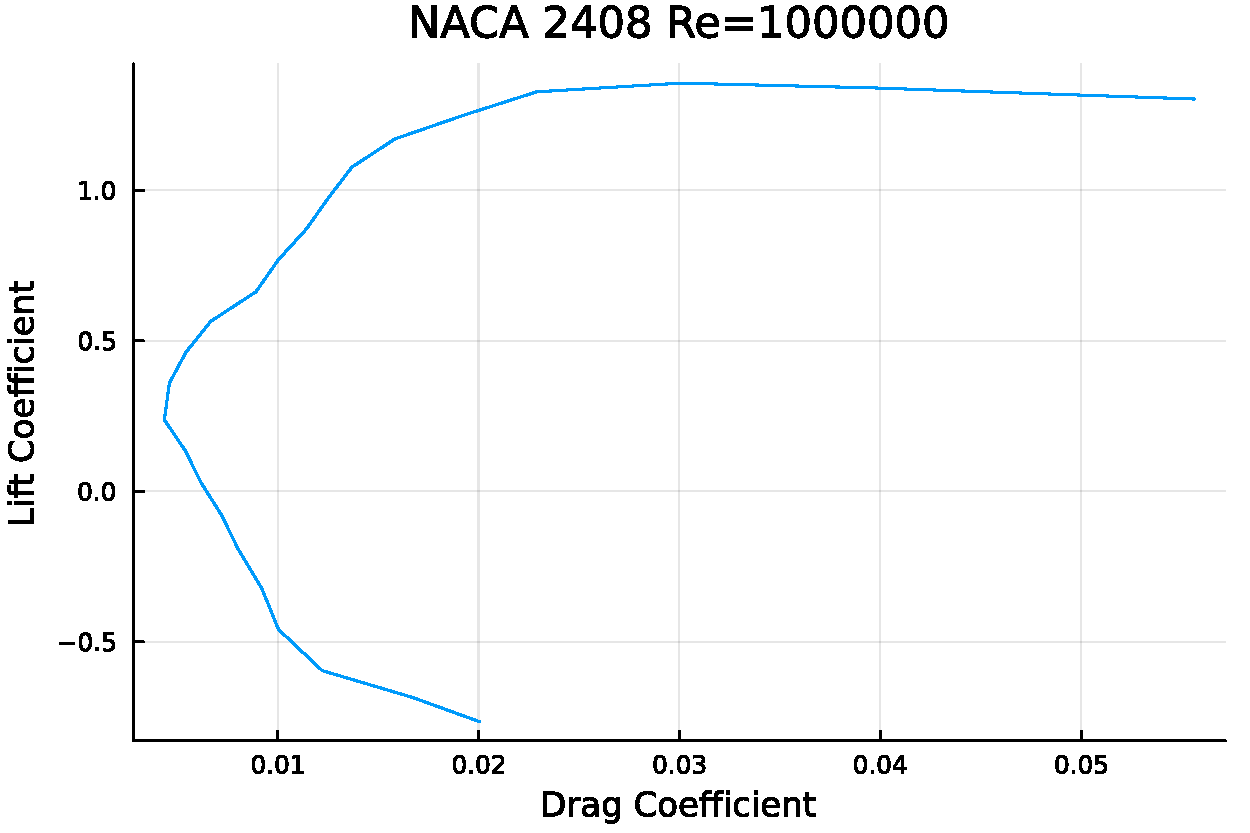
\includegraphics[width=\textwidth]{NACA 2408 Re=1000000_Drag_vs_Lift_Coefficent_Plot.pdf}
\caption{\label{fig:NACA 2408 Drag Lift}Drag vs Lift Profile NACA 2408}
\end{minipage}
\begin{minipage}[b]{0.32\textwidth}
\centering
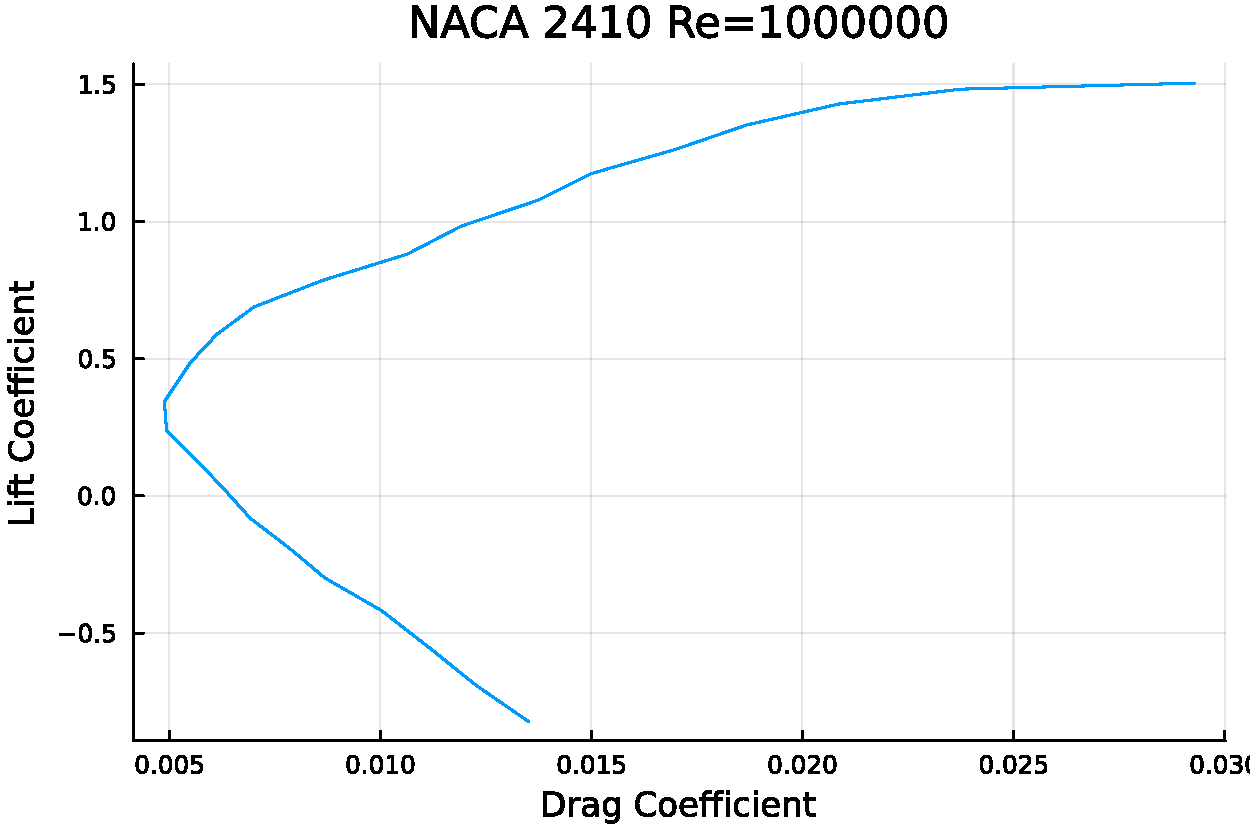
\includegraphics[width=\textwidth]{NACA 2410 Re=1000000_Drag_vs_Lift_Coefficent_Plot.pdf}
\caption{\label{fig:NACA 2410 Drag Lift}Drag vs Lift Profile NACA 2410}
\end{minipage}
\begin{minipage}[b]{0.32\textwidth}
\centering
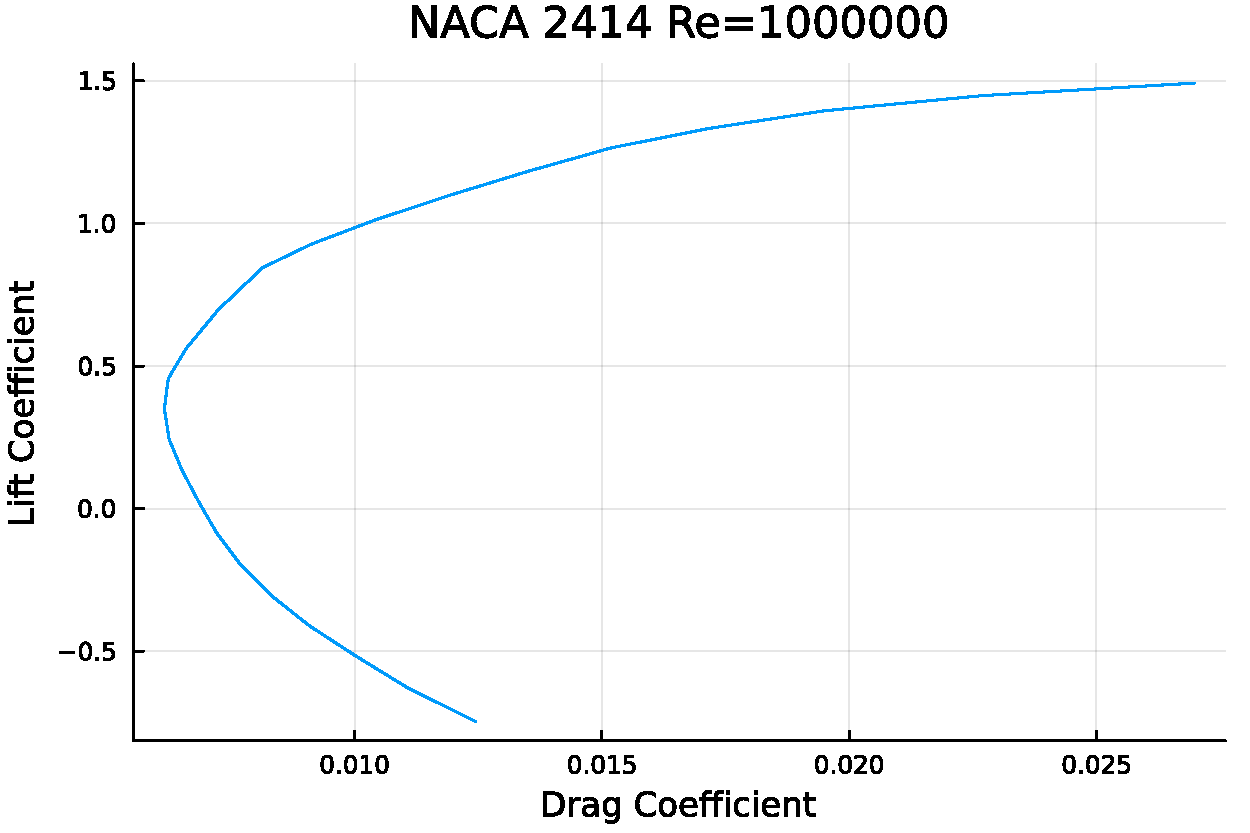
\includegraphics[width=\textwidth]{NACA 2414 Re=1000000_Drag_vs_Lift_Coefficent_Plot.pdf}
\caption{\label{fig:NACA 2414 Drag Lift}Drag vs Lift Profile NACA 2414}
\end{minipage}
\end{figure}

\clearpage

\section{Thickness Lift Curve Slope Plots}
\label{sec:third_appendix}

\begin{figure}[h]
    \centering
\begin{minipage}[b]{0.32\textwidth}
\centering
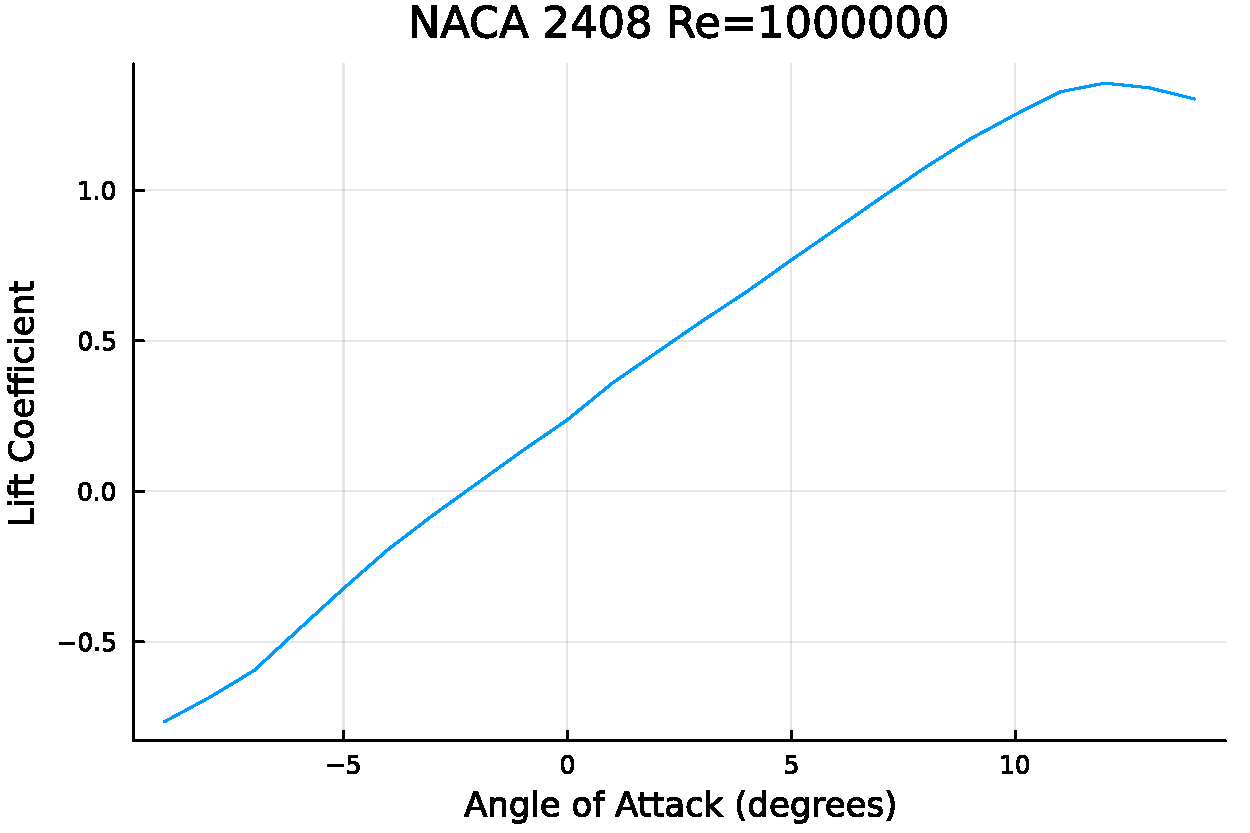
\includegraphics[width=\textwidth]{NACA 2408 Re=1000000_Lift_Coefficent_Plot.pdf}
\caption{\label{fig:NACA 2408 Lift}Drag vs Lift Profile NACA 2408}
\end{minipage}
\begin{minipage}[b]{0.32\textwidth}
\centering
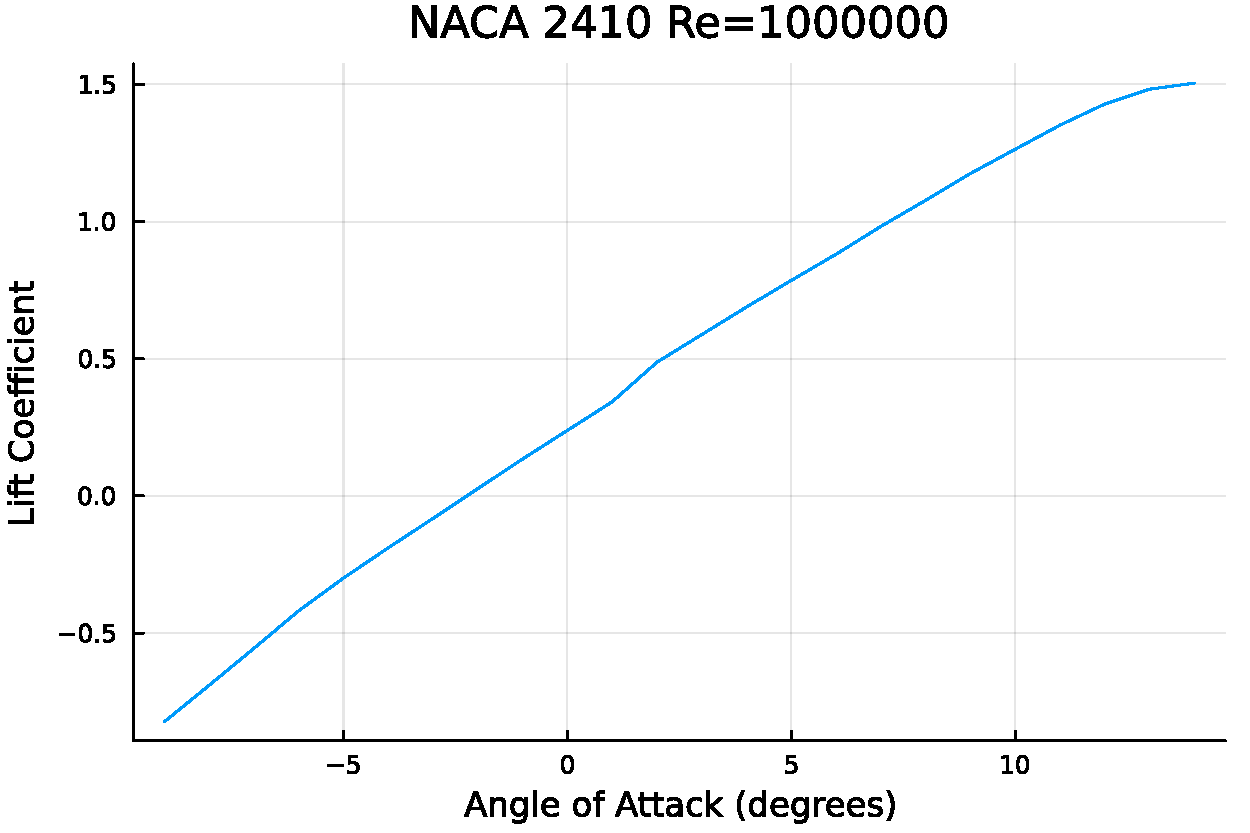
\includegraphics[width=\textwidth]{NACA 2410 Re=1000000_Lift_Coefficent_Plot.pdf}
\caption{\label{fig:NACA 2410 Lift}Drag vs Lift Profile NACA 2410}
\end{minipage}
\begin{minipage}[b]{0.32\textwidth}
\centering
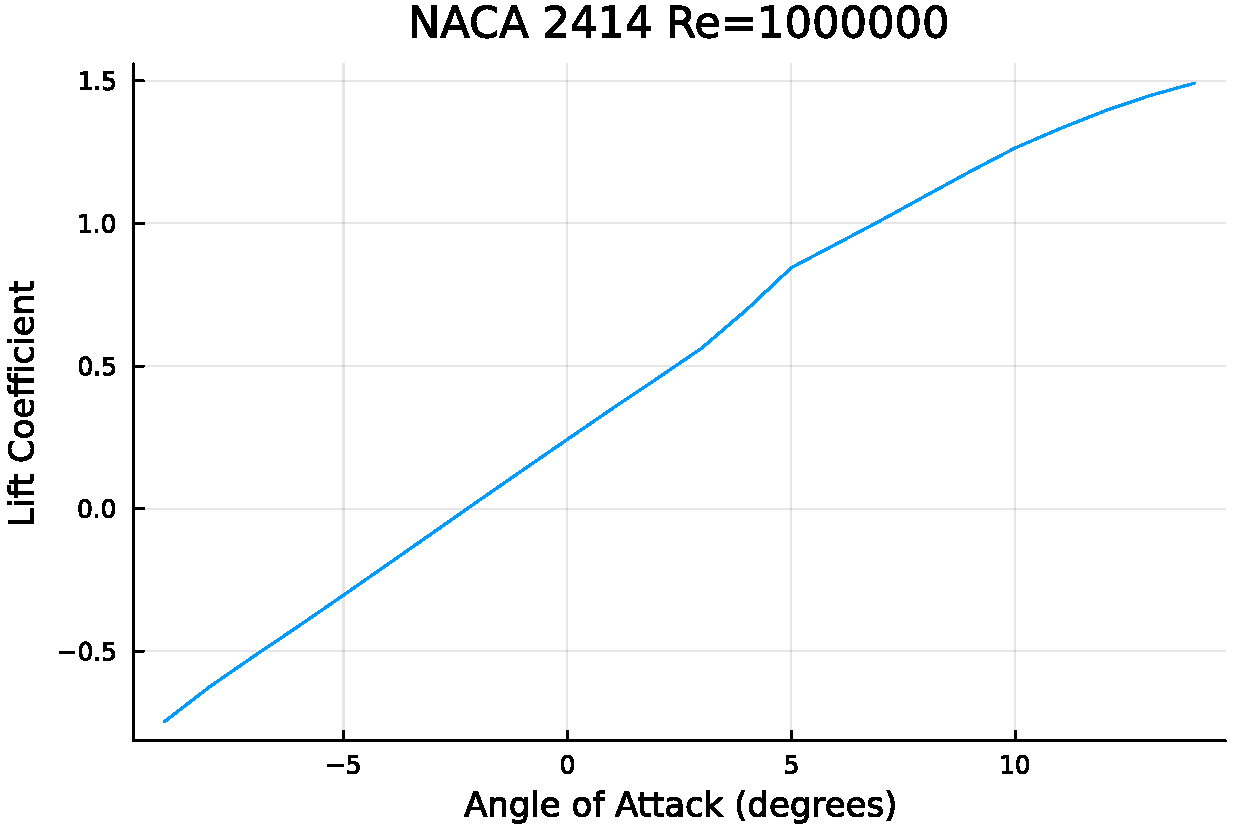
\includegraphics[width=\textwidth]{NACA 2414 Re=1000000_Lift_Coefficent_Plot.pdf}
\caption{\label{fig:NACA 2414 Lift}Drag vs Lift Profile NACA 2414}
\end{minipage}
\end{figure}


\end{document}